\chapter{Background}

\section{Terminology}
\subsection{What is serverless?}
\todo[inline]{Cite page 168 of wardley maps book}
Serverless computing emerged in the mid-to-late 2000s\cite{wardleyWardleyMaps2022,IntroducingGoogleApp,patilServerlessComputingEmergence2021} as a new paradigm for deploying applications, with the emergence of low-cost public cloud providers\cite{patilServerlessComputingEmergence2021,BenjaminBlackEC2}. It allows developers to deploy applications without managing the underlying infrastructure, leading to much more scalable and cost-effective solutions.

Typically, resources such as VMs\cite{hoeferTaxonomyCloudComputing2010} are rented in sub-second increments, and with storage and network charged by total usage. This results in a Pay-as-you-go (PAYG) model that can adapt to highly variable workloads\cite{sehgalCostBillingPractices2023,hilleyCloudComputingTaxonomy2009}.

Serverless applications are usually composed of cloud provider managed services, such as databases, storage, and compute, and are often event-driven\cite{EventarcOverview,EventListenerAmazon,robeceOverviewAzureEvent2024}. This means that application logic can be invoked by events, such as HTTP requests, database changes, or file uploads. This allows the application to scale independently\cite{goniwadaCloudNativeArchitecture2022}, as the cloud provider can provision resources as needed.

\subsection{What is a VM?}
\todo[inline]{Talk about how VMs act as an abstraction over physical hardware and can be provisioned to run applications. Typical startup times can vary based on how heavy-weight the VM is, typically ranging from seconds to minutes.}

\subsection{What is a container?}
\todo[inline]{Introduce containers as now the defacto standard of deployment of applications to cloud and serverless environments.}

\subsubsection{CGroups and Namespaces}
\todo[inline]{Talk about: CGroups, Namespaces and how they provide isolation mechanisms for containers.}

\subsubsection{Container Runtimes}
\todo[inline]{Talk about: runC, rkt, containerd, lxc.}

\subsection{What is \faas{}?}
Derived from the success of serverless computing, \faas{} rose to prominence in the mid-2010s\cite{AmazonWebServices2014,azureAnnouncingGeneralAvailability2016}. It allows developers to write code as functions that are executed in sandboxed environments in response to events, such as HTTP requests, database changes, or file uploads\cite{EventarcOverview,EventListenerAmazon,robeceOverviewAzureEvent2024}. Typically, serverless functions are billed for the duration of their execution in addition to a flat invocation cost, allowing for fine-grained billing of resources\cite{bortoliniInvestigatingPerformanceCost2020}. Additionally, since the underlying infrastructure of the function is abstracted away from the developer, the responsibility for scaling the function is moved to the cloud provider.

\section{\faas{} isolation mechanisms}
Typically, multi-tenany public \faas{} providers can be characterised into two categories: providers offering VM based isolation\cite{agacheFirecrackerLightweightVirtualization2020} and providers offering container based isolation\cite{GVisor}. Both types provide differing levels of security guarantees, and have different performance characteristics.

\subsection{VM based isolation}
VM based isolation is typically considered a much more secure form of isolation between \faas{} functions on multitenant public clouds\cite{jithinVirtualMachineIsolation2014}, however it typically has the highest overhead, since each function runs in its own virtual machine, with its own kernel. This overhead usually manifests in higher cold start times, however there has been considerable work carried out to reduce this overhead\cite{razaviPrebakedUVMsScalable2015,agacheFirecrackerLightweightVirtualization2020,dawXanaduMitigatingCascading2020,oliverstenbomRefunctionEliminatingServerless2019}.

Kata Containers\cite{KataContainersOpen} provides a container-like interface to VMs, interfacing with existing hypervisors such as Firecracker\cite{agacheFirecrackerLightweightVirtualization2020}, QEMU\cite{QEMU} and Cloud Hypervisor\cite{CloudhypervisorCloudhypervisorVirtual} (previously NEMU\cite{IntelNemu2024}).

Firecracker \cite{agacheFirecrackerLightweightVirtualization2020} is a lightweight KVM\cite{KVM} based Virtual Machine Monitor (VMM) allowing MicroVM provisioning in the order of \qtyrange{125}{150}{\ms} that provides a secure and fast environment for running \faas{} functions.

MicroVMs are intended to be lightweight, and provide a secure environment for running functions, with a fast boot time. Firecracker is written in Rust and unlike QEMU, provides secure, fast and stripped back devices to the guest VM in order to both reduce the attack surface and improve performance\cite{jainStudyFirecrackerMicroVM2020}.

LightVM redesigns the Xen Hypervisor's control plane such that VMs can boot in the order of \qtyrange{2}{3}{\ms}\cite{mancoMyVMLighter2017}, and achieveing a much higher VM density on a host.

\subsection{Container based isolation}
In contrast to VM based isolation, container based isolation is typically considered to be less secure\cite{DemystifyingContainerVs}, however it has a much lower overhead, since each function runs in its own container sharing a kernel with the host\cite{WhatContainerDocker}. From a security perspective, any kernel vulnerabilities could potentially be exploited by a malicious container to escape the sandbox and gain access to the host\cite{linMeasurementStudyLinux2018}.

GVisor is a container runtime that aims to improve security for running containers in a multitenant environment\cite{GVisor}. It implements a userspace `application kernel' that intercepts system calls made by untrusted container, providing a layer of abstraction between any possible vulnerabilities in the host kernel and the code executing in the untrusted container.

Whilst cold-start times of container-based \faas{} isolation are considerably lower than VM based isolation methods, cold-starts times can vary based on a variety of factors. SOCK reduces cold-start times by caching common dependencies in container images, reducing the image footprint and improving cold start times\cite{oakesSOCKRapidTask2018}. Refunction reuses containers between function invocations, reducing cold start times\cite{oliverstenbomRefunctionEliminatingServerless2019}. Pegurus also reuses warm containers between different function invocations to reduce cold start times\cite{liPagurusEliminatingCold2021}. Xanadu reduces cold start times by pre-warming containers based on a predictive model that estimates which subsequent functions will be triggered in a \faas{} workflow\cite{dawXanaduMitigatingCascading2020}.

\subsection{V8 isolate based isolation}
Whilst containers provide a much lighter footprint in comparison to VM based isolation, CloudFlare Workers\cite{CloudComputingContainers2018} and Vercel Edge Functions\cite{EdgeRuntime} both utilise V8 isolates to provide lightweight user-space isolation between functions. Whilst less secure than process-based isolation employed by contianers, V8 isolates provide a much denser packing of functions on a single host, and can provide much lower cold start times.

Additional work surrounding microarchitectural vulnerabilities such as Spectre within V8 isolates has been carried out to ensure that V8 isolates can execute securely in multitenant environment\cite{schwarzlRobustScalableProcess2022}.

Apache OpenWhisk\cite{apacheOpenWhisk2024} is an open-source \faas{} platform that provides container based isolation, leveraging Nginx as an HTTP gateway, Kafka as a message broker to queue invocations, CouchDB as a persistent data storage layer and OCI containers to execute arbitrary function logic.

OpenFaaS\cite{ellisOpenFaaS2024} provides container based isolation for \faas{} using Kubernetes to handle scaling and execution of functions, and Prometheus to handle scaling of the functions.

\subsection{GraalOS and GraalVM based isolation}
\todo[inline]{Discuss how GraalOS and GraalVM reduces cold start times.}

\subsection{Wasm based isolation}
WASM provides a secure and efficient environment for executing untrusted code\cite{WebAssembly} in a multitenant environment. Initially developed to run in the browser, WASM allows for the execution of untrusted code in a sandboxed environment without the need for a full VM or container. It has formal semantics\cite{haasBringingWebSpeed2017}, its embeddings can be formally proven to be memory-safe\cite{SecurefoundationsVWasm2024}, and utilises software based fault isolation to ensure that code cannot escape the sandbox\cite{SecurityWebAssembly}. Despite this effort, microarchitectural vulnerabilities such as Spectre still exist within WASM runtimes, and additional work is being carried out to mitigate these\cite{narayanSwivelHardeningWebAssembly2021}.

Fastly Edge Compute Platform\cite{EdgeCloudPlatform} utilises Lucet\cite{BytecodeallianceLucet2024} (now Wasmtime\cite{Wasmtime}) to sandbox WebAssembly executables from one-another. Fastly Edge Compute Platform cites startup times in the order of tens of microseconds to instantiate the sandbox.

In addition to JavaScript functions deployed using V8 isolates, Cloudflare Workers\cite{CloudComputingContainers2018} also allow WASM based functions to be deployed to their edge network. Unlike Fastly, Cloudflare Workers do not execute the function within a WASM runtime, and instead rely on the V8 runtime to execute WASM functions\cite{WebAssemblyWasmCloudflare2024}.

Sledge reduces cold-start times and increases throughput over other WASM based \faas{} frameworks by leveraging LLVM to compile WASM binaries, specifically targetting edge hardware and implements user-space scheduling of functions\cite{gadepalliSledgeServerlessfirstLightweight2020}.

FaaSM employs a similar approach to container based isolation, using CGroups and Namespaces for isolation, and executing WASM binaries. In order to improve interprocess communication and persisting state, FaaSM utilises shared memory to allow functions to communicate with one another\cite{shillakerFaasmLightweightIsolation2020}.

\section{\faas{} billing models}
\label{sec:faas-billing-models}

The \faas{} billing model is a complex model built around a number of factors that vary between cloud providers. Despite their intricacies and differences, the prevailing common billing model, referred to in Equation \ref{eq:faas-billing-model} can be characterised by a function of: a flat-rate invocation cost ($C_i$), and a rate ($C_r$) per unit of time ($G$) charged over the total invocation time ($t$), from the start of a function to the point at which it returns a response, with a minimum billable cost $C_{min}$.

\begin{equation} \label{eq:faas-billing-model}
C_t = C_i + \max\left(C_{min},\ceil*{\frac{t}{G}} C_r\right)
\end{equation}

All the major cloud providers scale their charged rate per unit of time linearly with resource allocation.

Billing cost curves for function resource allocations of \SI{128}{\mega\byte}, \SI{256}{\mega\byte} and \SI{512}{\mega\byte} respectively on each of the three major cloud platforms are shown in Figure \ref{fig:faas-billing-cost-curves}. Notice that the cost curves for AWS Lambda are linear since they have no minimum billable cost, whereas Azure Functions and Google Cloud Functions have a minimum billable cost, resulting in a flat initial cost for the first \SI{100}{\milli\second}.

\begin{figure*}[htp]
    \centering
    \subfigure[AWS Lambda billing cost curve]{
        \centering
        %% Creator: Matplotlib, PGF backend
%%
%% To include the figure in your LaTeX document, write
%%   \input{<filename>.pgf}
%%
%% Make sure the required packages are loaded in your preamble
%%   \usepackage{pgf}
%%
%% Also ensure that all the required font packages are loaded; for instance,
%% the lmodern package is sometimes necessary when using math font.
%%   \usepackage{lmodern}
%%
%% Figures using additional raster images can only be included by \input if
%% they are in the same directory as the main LaTeX file. For loading figures
%% from other directories you can use the `import` package
%%   \usepackage{import}
%%
%% and then include the figures with
%%   \import{<path to file>}{<filename>.pgf}
%%
%% Matplotlib used the following preamble
%%   \def\mathdefault#1{#1}
%%   \everymath=\expandafter{\the\everymath\displaystyle}
%%   
%%   \makeatletter\@ifpackageloaded{underscore}{}{\usepackage[strings]{underscore}}\makeatother
%%
\begingroup%
\makeatletter%
\begin{pgfpicture}%
\pgfpathrectangle{\pgfpointorigin}{\pgfqpoint{2.847846in}{3.785303in}}%
\pgfusepath{use as bounding box, clip}%
\begin{pgfscope}%
\pgfsetbuttcap%
\pgfsetmiterjoin%
\definecolor{currentfill}{rgb}{1.000000,1.000000,1.000000}%
\pgfsetfillcolor{currentfill}%
\pgfsetlinewidth{0.000000pt}%
\definecolor{currentstroke}{rgb}{1.000000,1.000000,1.000000}%
\pgfsetstrokecolor{currentstroke}%
\pgfsetdash{}{0pt}%
\pgfpathmoveto{\pgfqpoint{0.000000in}{0.000000in}}%
\pgfpathlineto{\pgfqpoint{2.847846in}{0.000000in}}%
\pgfpathlineto{\pgfqpoint{2.847846in}{3.785303in}}%
\pgfpathlineto{\pgfqpoint{0.000000in}{3.785303in}}%
\pgfpathlineto{\pgfqpoint{0.000000in}{0.000000in}}%
\pgfpathclose%
\pgfusepath{fill}%
\end{pgfscope}%
\begin{pgfscope}%
\pgfsetbuttcap%
\pgfsetmiterjoin%
\definecolor{currentfill}{rgb}{0.917647,0.917647,0.949020}%
\pgfsetfillcolor{currentfill}%
\pgfsetlinewidth{0.000000pt}%
\definecolor{currentstroke}{rgb}{0.000000,0.000000,0.000000}%
\pgfsetstrokecolor{currentstroke}%
\pgfsetstrokeopacity{0.000000}%
\pgfsetdash{}{0pt}%
\pgfpathmoveto{\pgfqpoint{0.648496in}{0.589352in}}%
\pgfpathlineto{\pgfqpoint{2.715111in}{0.589352in}}%
\pgfpathlineto{\pgfqpoint{2.715111in}{3.327062in}}%
\pgfpathlineto{\pgfqpoint{0.648496in}{3.327062in}}%
\pgfpathlineto{\pgfqpoint{0.648496in}{0.589352in}}%
\pgfpathclose%
\pgfusepath{fill}%
\end{pgfscope}%
\begin{pgfscope}%
\pgfpathrectangle{\pgfqpoint{0.648496in}{0.589352in}}{\pgfqpoint{2.066616in}{2.737710in}}%
\pgfusepath{clip}%
\pgfsetroundcap%
\pgfsetroundjoin%
\pgfsetlinewidth{1.003750pt}%
\definecolor{currentstroke}{rgb}{1.000000,1.000000,1.000000}%
\pgfsetstrokecolor{currentstroke}%
\pgfsetdash{}{0pt}%
\pgfpathmoveto{\pgfqpoint{0.742433in}{0.589352in}}%
\pgfpathlineto{\pgfqpoint{0.742433in}{3.327062in}}%
\pgfusepath{stroke}%
\end{pgfscope}%
\begin{pgfscope}%
\definecolor{textcolor}{rgb}{0.150000,0.150000,0.150000}%
\pgfsetstrokecolor{textcolor}%
\pgfsetfillcolor{textcolor}%
\pgftext[x=0.742433in,y=0.457407in,,top]{\color{textcolor}{\rmfamily\fontsize{11.000000}{13.200000}\selectfont\catcode`\^=\active\def^{\ifmmode\sp\else\^{}\fi}\catcode`\%=\active\def%{\%}$\mathdefault{0}$}}%
\end{pgfscope}%
\begin{pgfscope}%
\pgfpathrectangle{\pgfqpoint{0.648496in}{0.589352in}}{\pgfqpoint{2.066616in}{2.737710in}}%
\pgfusepath{clip}%
\pgfsetroundcap%
\pgfsetroundjoin%
\pgfsetlinewidth{1.003750pt}%
\definecolor{currentstroke}{rgb}{1.000000,1.000000,1.000000}%
\pgfsetstrokecolor{currentstroke}%
\pgfsetdash{}{0pt}%
\pgfpathmoveto{\pgfqpoint{1.372883in}{0.589352in}}%
\pgfpathlineto{\pgfqpoint{1.372883in}{3.327062in}}%
\pgfusepath{stroke}%
\end{pgfscope}%
\begin{pgfscope}%
\definecolor{textcolor}{rgb}{0.150000,0.150000,0.150000}%
\pgfsetstrokecolor{textcolor}%
\pgfsetfillcolor{textcolor}%
\pgftext[x=1.372883in,y=0.457407in,,top]{\color{textcolor}{\rmfamily\fontsize{11.000000}{13.200000}\selectfont\catcode`\^=\active\def^{\ifmmode\sp\else\^{}\fi}\catcode`\%=\active\def%{\%}$\mathdefault{50}$}}%
\end{pgfscope}%
\begin{pgfscope}%
\pgfpathrectangle{\pgfqpoint{0.648496in}{0.589352in}}{\pgfqpoint{2.066616in}{2.737710in}}%
\pgfusepath{clip}%
\pgfsetroundcap%
\pgfsetroundjoin%
\pgfsetlinewidth{1.003750pt}%
\definecolor{currentstroke}{rgb}{1.000000,1.000000,1.000000}%
\pgfsetstrokecolor{currentstroke}%
\pgfsetdash{}{0pt}%
\pgfpathmoveto{\pgfqpoint{2.003333in}{0.589352in}}%
\pgfpathlineto{\pgfqpoint{2.003333in}{3.327062in}}%
\pgfusepath{stroke}%
\end{pgfscope}%
\begin{pgfscope}%
\definecolor{textcolor}{rgb}{0.150000,0.150000,0.150000}%
\pgfsetstrokecolor{textcolor}%
\pgfsetfillcolor{textcolor}%
\pgftext[x=2.003333in,y=0.457407in,,top]{\color{textcolor}{\rmfamily\fontsize{11.000000}{13.200000}\selectfont\catcode`\^=\active\def^{\ifmmode\sp\else\^{}\fi}\catcode`\%=\active\def%{\%}$\mathdefault{100}$}}%
\end{pgfscope}%
\begin{pgfscope}%
\pgfpathrectangle{\pgfqpoint{0.648496in}{0.589352in}}{\pgfqpoint{2.066616in}{2.737710in}}%
\pgfusepath{clip}%
\pgfsetroundcap%
\pgfsetroundjoin%
\pgfsetlinewidth{1.003750pt}%
\definecolor{currentstroke}{rgb}{1.000000,1.000000,1.000000}%
\pgfsetstrokecolor{currentstroke}%
\pgfsetdash{}{0pt}%
\pgfpathmoveto{\pgfqpoint{2.633783in}{0.589352in}}%
\pgfpathlineto{\pgfqpoint{2.633783in}{3.327062in}}%
\pgfusepath{stroke}%
\end{pgfscope}%
\begin{pgfscope}%
\definecolor{textcolor}{rgb}{0.150000,0.150000,0.150000}%
\pgfsetstrokecolor{textcolor}%
\pgfsetfillcolor{textcolor}%
\pgftext[x=2.633783in,y=0.457407in,,top]{\color{textcolor}{\rmfamily\fontsize{11.000000}{13.200000}\selectfont\catcode`\^=\active\def^{\ifmmode\sp\else\^{}\fi}\catcode`\%=\active\def%{\%}$\mathdefault{150}$}}%
\end{pgfscope}%
\begin{pgfscope}%
\definecolor{textcolor}{rgb}{0.150000,0.150000,0.150000}%
\pgfsetstrokecolor{textcolor}%
\pgfsetfillcolor{textcolor}%
\pgftext[x=1.681803in,y=0.266667in,,top]{\color{textcolor}{\rmfamily\fontsize{12.000000}{14.400000}\selectfont\catcode`\^=\active\def^{\ifmmode\sp\else\^{}\fi}\catcode`\%=\active\def%{\%}Time (ms)}}%
\end{pgfscope}%
\begin{pgfscope}%
\pgfpathrectangle{\pgfqpoint{0.648496in}{0.589352in}}{\pgfqpoint{2.066616in}{2.737710in}}%
\pgfusepath{clip}%
\pgfsetroundcap%
\pgfsetroundjoin%
\pgfsetlinewidth{1.003750pt}%
\definecolor{currentstroke}{rgb}{1.000000,1.000000,1.000000}%
\pgfsetstrokecolor{currentstroke}%
\pgfsetdash{}{0pt}%
\pgfpathmoveto{\pgfqpoint{0.648496in}{0.713793in}}%
\pgfpathlineto{\pgfqpoint{2.715111in}{0.713793in}}%
\pgfusepath{stroke}%
\end{pgfscope}%
\begin{pgfscope}%
\definecolor{textcolor}{rgb}{0.150000,0.150000,0.150000}%
\pgfsetstrokecolor{textcolor}%
\pgfsetfillcolor{textcolor}%
\pgftext[x=0.322222in, y=0.660987in, left, base]{\color{textcolor}{\rmfamily\fontsize{11.000000}{13.200000}\selectfont\catcode`\^=\active\def^{\ifmmode\sp\else\^{}\fi}\catcode`\%=\active\def%{\%}$\mathdefault{0.0}$}}%
\end{pgfscope}%
\begin{pgfscope}%
\pgfpathrectangle{\pgfqpoint{0.648496in}{0.589352in}}{\pgfqpoint{2.066616in}{2.737710in}}%
\pgfusepath{clip}%
\pgfsetroundcap%
\pgfsetroundjoin%
\pgfsetlinewidth{1.003750pt}%
\definecolor{currentstroke}{rgb}{1.000000,1.000000,1.000000}%
\pgfsetstrokecolor{currentstroke}%
\pgfsetdash{}{0pt}%
\pgfpathmoveto{\pgfqpoint{0.648496in}{1.059063in}}%
\pgfpathlineto{\pgfqpoint{2.715111in}{1.059063in}}%
\pgfusepath{stroke}%
\end{pgfscope}%
\begin{pgfscope}%
\definecolor{textcolor}{rgb}{0.150000,0.150000,0.150000}%
\pgfsetstrokecolor{textcolor}%
\pgfsetfillcolor{textcolor}%
\pgftext[x=0.322222in, y=1.006257in, left, base]{\color{textcolor}{\rmfamily\fontsize{11.000000}{13.200000}\selectfont\catcode`\^=\active\def^{\ifmmode\sp\else\^{}\fi}\catcode`\%=\active\def%{\%}$\mathdefault{0.2}$}}%
\end{pgfscope}%
\begin{pgfscope}%
\pgfpathrectangle{\pgfqpoint{0.648496in}{0.589352in}}{\pgfqpoint{2.066616in}{2.737710in}}%
\pgfusepath{clip}%
\pgfsetroundcap%
\pgfsetroundjoin%
\pgfsetlinewidth{1.003750pt}%
\definecolor{currentstroke}{rgb}{1.000000,1.000000,1.000000}%
\pgfsetstrokecolor{currentstroke}%
\pgfsetdash{}{0pt}%
\pgfpathmoveto{\pgfqpoint{0.648496in}{1.404334in}}%
\pgfpathlineto{\pgfqpoint{2.715111in}{1.404334in}}%
\pgfusepath{stroke}%
\end{pgfscope}%
\begin{pgfscope}%
\definecolor{textcolor}{rgb}{0.150000,0.150000,0.150000}%
\pgfsetstrokecolor{textcolor}%
\pgfsetfillcolor{textcolor}%
\pgftext[x=0.322222in, y=1.351527in, left, base]{\color{textcolor}{\rmfamily\fontsize{11.000000}{13.200000}\selectfont\catcode`\^=\active\def^{\ifmmode\sp\else\^{}\fi}\catcode`\%=\active\def%{\%}$\mathdefault{0.4}$}}%
\end{pgfscope}%
\begin{pgfscope}%
\pgfpathrectangle{\pgfqpoint{0.648496in}{0.589352in}}{\pgfqpoint{2.066616in}{2.737710in}}%
\pgfusepath{clip}%
\pgfsetroundcap%
\pgfsetroundjoin%
\pgfsetlinewidth{1.003750pt}%
\definecolor{currentstroke}{rgb}{1.000000,1.000000,1.000000}%
\pgfsetstrokecolor{currentstroke}%
\pgfsetdash{}{0pt}%
\pgfpathmoveto{\pgfqpoint{0.648496in}{1.749604in}}%
\pgfpathlineto{\pgfqpoint{2.715111in}{1.749604in}}%
\pgfusepath{stroke}%
\end{pgfscope}%
\begin{pgfscope}%
\definecolor{textcolor}{rgb}{0.150000,0.150000,0.150000}%
\pgfsetstrokecolor{textcolor}%
\pgfsetfillcolor{textcolor}%
\pgftext[x=0.322222in, y=1.696797in, left, base]{\color{textcolor}{\rmfamily\fontsize{11.000000}{13.200000}\selectfont\catcode`\^=\active\def^{\ifmmode\sp\else\^{}\fi}\catcode`\%=\active\def%{\%}$\mathdefault{0.6}$}}%
\end{pgfscope}%
\begin{pgfscope}%
\pgfpathrectangle{\pgfqpoint{0.648496in}{0.589352in}}{\pgfqpoint{2.066616in}{2.737710in}}%
\pgfusepath{clip}%
\pgfsetroundcap%
\pgfsetroundjoin%
\pgfsetlinewidth{1.003750pt}%
\definecolor{currentstroke}{rgb}{1.000000,1.000000,1.000000}%
\pgfsetstrokecolor{currentstroke}%
\pgfsetdash{}{0pt}%
\pgfpathmoveto{\pgfqpoint{0.648496in}{2.094874in}}%
\pgfpathlineto{\pgfqpoint{2.715111in}{2.094874in}}%
\pgfusepath{stroke}%
\end{pgfscope}%
\begin{pgfscope}%
\definecolor{textcolor}{rgb}{0.150000,0.150000,0.150000}%
\pgfsetstrokecolor{textcolor}%
\pgfsetfillcolor{textcolor}%
\pgftext[x=0.322222in, y=2.042068in, left, base]{\color{textcolor}{\rmfamily\fontsize{11.000000}{13.200000}\selectfont\catcode`\^=\active\def^{\ifmmode\sp\else\^{}\fi}\catcode`\%=\active\def%{\%}$\mathdefault{0.8}$}}%
\end{pgfscope}%
\begin{pgfscope}%
\pgfpathrectangle{\pgfqpoint{0.648496in}{0.589352in}}{\pgfqpoint{2.066616in}{2.737710in}}%
\pgfusepath{clip}%
\pgfsetroundcap%
\pgfsetroundjoin%
\pgfsetlinewidth{1.003750pt}%
\definecolor{currentstroke}{rgb}{1.000000,1.000000,1.000000}%
\pgfsetstrokecolor{currentstroke}%
\pgfsetdash{}{0pt}%
\pgfpathmoveto{\pgfqpoint{0.648496in}{2.440145in}}%
\pgfpathlineto{\pgfqpoint{2.715111in}{2.440145in}}%
\pgfusepath{stroke}%
\end{pgfscope}%
\begin{pgfscope}%
\definecolor{textcolor}{rgb}{0.150000,0.150000,0.150000}%
\pgfsetstrokecolor{textcolor}%
\pgfsetfillcolor{textcolor}%
\pgftext[x=0.322222in, y=2.387338in, left, base]{\color{textcolor}{\rmfamily\fontsize{11.000000}{13.200000}\selectfont\catcode`\^=\active\def^{\ifmmode\sp\else\^{}\fi}\catcode`\%=\active\def%{\%}$\mathdefault{1.0}$}}%
\end{pgfscope}%
\begin{pgfscope}%
\pgfpathrectangle{\pgfqpoint{0.648496in}{0.589352in}}{\pgfqpoint{2.066616in}{2.737710in}}%
\pgfusepath{clip}%
\pgfsetroundcap%
\pgfsetroundjoin%
\pgfsetlinewidth{1.003750pt}%
\definecolor{currentstroke}{rgb}{1.000000,1.000000,1.000000}%
\pgfsetstrokecolor{currentstroke}%
\pgfsetdash{}{0pt}%
\pgfpathmoveto{\pgfqpoint{0.648496in}{2.785415in}}%
\pgfpathlineto{\pgfqpoint{2.715111in}{2.785415in}}%
\pgfusepath{stroke}%
\end{pgfscope}%
\begin{pgfscope}%
\definecolor{textcolor}{rgb}{0.150000,0.150000,0.150000}%
\pgfsetstrokecolor{textcolor}%
\pgfsetfillcolor{textcolor}%
\pgftext[x=0.322222in, y=2.732608in, left, base]{\color{textcolor}{\rmfamily\fontsize{11.000000}{13.200000}\selectfont\catcode`\^=\active\def^{\ifmmode\sp\else\^{}\fi}\catcode`\%=\active\def%{\%}$\mathdefault{1.2}$}}%
\end{pgfscope}%
\begin{pgfscope}%
\pgfpathrectangle{\pgfqpoint{0.648496in}{0.589352in}}{\pgfqpoint{2.066616in}{2.737710in}}%
\pgfusepath{clip}%
\pgfsetroundcap%
\pgfsetroundjoin%
\pgfsetlinewidth{1.003750pt}%
\definecolor{currentstroke}{rgb}{1.000000,1.000000,1.000000}%
\pgfsetstrokecolor{currentstroke}%
\pgfsetdash{}{0pt}%
\pgfpathmoveto{\pgfqpoint{0.648496in}{3.130685in}}%
\pgfpathlineto{\pgfqpoint{2.715111in}{3.130685in}}%
\pgfusepath{stroke}%
\end{pgfscope}%
\begin{pgfscope}%
\definecolor{textcolor}{rgb}{0.150000,0.150000,0.150000}%
\pgfsetstrokecolor{textcolor}%
\pgfsetfillcolor{textcolor}%
\pgftext[x=0.322222in, y=3.077879in, left, base]{\color{textcolor}{\rmfamily\fontsize{11.000000}{13.200000}\selectfont\catcode`\^=\active\def^{\ifmmode\sp\else\^{}\fi}\catcode`\%=\active\def%{\%}$\mathdefault{1.4}$}}%
\end{pgfscope}%
\begin{pgfscope}%
\definecolor{textcolor}{rgb}{0.150000,0.150000,0.150000}%
\pgfsetstrokecolor{textcolor}%
\pgfsetfillcolor{textcolor}%
\pgftext[x=0.266667in,y=1.958207in,,bottom,rotate=90.000000]{\color{textcolor}{\rmfamily\fontsize{12.000000}{14.400000}\selectfont\catcode`\^=\active\def^{\ifmmode\sp\else\^{}\fi}\catcode`\%=\active\def%{\%}Price (USD)}}%
\end{pgfscope}%
\begin{pgfscope}%
\definecolor{textcolor}{rgb}{0.150000,0.150000,0.150000}%
\pgfsetstrokecolor{textcolor}%
\pgfsetfillcolor{textcolor}%
\pgftext[x=0.648496in,y=3.368729in,left,base]{\color{textcolor}{\rmfamily\fontsize{11.000000}{13.200000}\selectfont\catcode`\^=\active\def^{\ifmmode\sp\else\^{}\fi}\catcode`\%=\active\def%{\%}$\times\mathdefault{10^{\ensuremath{-}6}}\mathdefault{}$}}%
\end{pgfscope}%
\begin{pgfscope}%
\pgfpathrectangle{\pgfqpoint{0.648496in}{0.589352in}}{\pgfqpoint{2.066616in}{2.737710in}}%
\pgfusepath{clip}%
\pgfsetbuttcap%
\pgfsetmiterjoin%
\definecolor{currentfill}{rgb}{0.768627,0.305882,0.321569}%
\pgfsetfillcolor{currentfill}%
\pgfsetfillopacity{0.200000}%
\pgfsetlinewidth{1.003750pt}%
\definecolor{currentstroke}{rgb}{0.768627,0.305882,0.321569}%
\pgfsetstrokecolor{currentstroke}%
\pgfsetstrokeopacity{0.200000}%
\pgfsetdash{}{0pt}%
\pgfpathmoveto{\pgfqpoint{0.648496in}{0.713793in}}%
\pgfpathlineto{\pgfqpoint{0.648496in}{1.059063in}}%
\pgfpathlineto{\pgfqpoint{2.715111in}{1.059063in}}%
\pgfpathlineto{\pgfqpoint{2.715111in}{0.713793in}}%
\pgfpathlineto{\pgfqpoint{0.648496in}{0.713793in}}%
\pgfpathclose%
\pgfusepath{stroke,fill}%
\end{pgfscope}%
\begin{pgfscope}%
\pgfpathrectangle{\pgfqpoint{0.648496in}{0.589352in}}{\pgfqpoint{2.066616in}{2.737710in}}%
\pgfusepath{clip}%
\pgfsetroundcap%
\pgfsetroundjoin%
\pgfsetlinewidth{1.505625pt}%
\definecolor{currentstroke}{rgb}{0.298039,0.447059,0.690196}%
\pgfsetstrokecolor{currentstroke}%
\pgfsetdash{}{0pt}%
\pgfpathmoveto{\pgfqpoint{0.742433in}{1.059063in}}%
\pgfpathlineto{\pgfqpoint{2.621174in}{1.594953in}}%
\pgfpathlineto{\pgfqpoint{2.621174in}{1.594953in}}%
\pgfusepath{stroke}%
\end{pgfscope}%
\begin{pgfscope}%
\pgfpathrectangle{\pgfqpoint{0.648496in}{0.589352in}}{\pgfqpoint{2.066616in}{2.737710in}}%
\pgfusepath{clip}%
\pgfsetroundcap%
\pgfsetroundjoin%
\pgfsetlinewidth{1.505625pt}%
\definecolor{currentstroke}{rgb}{0.866667,0.517647,0.321569}%
\pgfsetstrokecolor{currentstroke}%
\pgfsetdash{}{0pt}%
\pgfpathmoveto{\pgfqpoint{0.742433in}{1.059063in}}%
\pgfpathlineto{\pgfqpoint{2.621174in}{2.130842in}}%
\pgfpathlineto{\pgfqpoint{2.621174in}{2.130842in}}%
\pgfusepath{stroke}%
\end{pgfscope}%
\begin{pgfscope}%
\pgfpathrectangle{\pgfqpoint{0.648496in}{0.589352in}}{\pgfqpoint{2.066616in}{2.737710in}}%
\pgfusepath{clip}%
\pgfsetroundcap%
\pgfsetroundjoin%
\pgfsetlinewidth{1.505625pt}%
\definecolor{currentstroke}{rgb}{0.333333,0.658824,0.407843}%
\pgfsetstrokecolor{currentstroke}%
\pgfsetdash{}{0pt}%
\pgfpathmoveto{\pgfqpoint{0.742433in}{1.059063in}}%
\pgfpathlineto{\pgfqpoint{2.621174in}{3.202621in}}%
\pgfpathlineto{\pgfqpoint{2.621174in}{3.202621in}}%
\pgfusepath{stroke}%
\end{pgfscope}%
\begin{pgfscope}%
\pgfpathrectangle{\pgfqpoint{0.648496in}{0.589352in}}{\pgfqpoint{2.066616in}{2.737710in}}%
\pgfusepath{clip}%
\pgfsetbuttcap%
\pgfsetroundjoin%
\pgfsetlinewidth{1.505625pt}%
\definecolor{currentstroke}{rgb}{0.768627,0.305882,0.321569}%
\pgfsetstrokecolor{currentstroke}%
\pgfsetdash{{5.550000pt}{2.400000pt}}{0.000000pt}%
\pgfpathmoveto{\pgfqpoint{0.648496in}{1.059063in}}%
\pgfpathlineto{\pgfqpoint{2.715111in}{1.059063in}}%
\pgfusepath{stroke}%
\end{pgfscope}%
\begin{pgfscope}%
\pgfsetrectcap%
\pgfsetmiterjoin%
\pgfsetlinewidth{1.254687pt}%
\definecolor{currentstroke}{rgb}{1.000000,1.000000,1.000000}%
\pgfsetstrokecolor{currentstroke}%
\pgfsetdash{}{0pt}%
\pgfpathmoveto{\pgfqpoint{0.648496in}{0.589352in}}%
\pgfpathlineto{\pgfqpoint{0.648496in}{3.327062in}}%
\pgfusepath{stroke}%
\end{pgfscope}%
\begin{pgfscope}%
\pgfsetrectcap%
\pgfsetmiterjoin%
\pgfsetlinewidth{1.254687pt}%
\definecolor{currentstroke}{rgb}{1.000000,1.000000,1.000000}%
\pgfsetstrokecolor{currentstroke}%
\pgfsetdash{}{0pt}%
\pgfpathmoveto{\pgfqpoint{2.715111in}{0.589352in}}%
\pgfpathlineto{\pgfqpoint{2.715111in}{3.327062in}}%
\pgfusepath{stroke}%
\end{pgfscope}%
\begin{pgfscope}%
\pgfsetrectcap%
\pgfsetmiterjoin%
\pgfsetlinewidth{1.254687pt}%
\definecolor{currentstroke}{rgb}{1.000000,1.000000,1.000000}%
\pgfsetstrokecolor{currentstroke}%
\pgfsetdash{}{0pt}%
\pgfpathmoveto{\pgfqpoint{0.648496in}{0.589352in}}%
\pgfpathlineto{\pgfqpoint{2.715111in}{0.589352in}}%
\pgfusepath{stroke}%
\end{pgfscope}%
\begin{pgfscope}%
\pgfsetrectcap%
\pgfsetmiterjoin%
\pgfsetlinewidth{1.254687pt}%
\definecolor{currentstroke}{rgb}{1.000000,1.000000,1.000000}%
\pgfsetstrokecolor{currentstroke}%
\pgfsetdash{}{0pt}%
\pgfpathmoveto{\pgfqpoint{0.648496in}{3.327062in}}%
\pgfpathlineto{\pgfqpoint{2.715111in}{3.327062in}}%
\pgfusepath{stroke}%
\end{pgfscope}%
\begin{pgfscope}%
\definecolor{textcolor}{rgb}{0.150000,0.150000,0.150000}%
\pgfsetstrokecolor{textcolor}%
\pgfsetfillcolor{textcolor}%
\pgftext[x=1.681803in,y=3.569563in,,base]{\color{textcolor}{\rmfamily\fontsize{12.000000}{14.400000}\selectfont\catcode`\^=\active\def^{\ifmmode\sp\else\^{}\fi}\catcode`\%=\active\def%{\%}AWS Lambda Cost Curve}}%
\end{pgfscope}%
\begin{pgfscope}%
\pgfsetbuttcap%
\pgfsetmiterjoin%
\definecolor{currentfill}{rgb}{0.917647,0.917647,0.949020}%
\pgfsetfillcolor{currentfill}%
\pgfsetfillopacity{0.800000}%
\pgfsetlinewidth{1.003750pt}%
\definecolor{currentstroke}{rgb}{0.800000,0.800000,0.800000}%
\pgfsetstrokecolor{currentstroke}%
\pgfsetstrokeopacity{0.800000}%
\pgfsetdash{}{0pt}%
\pgfpathmoveto{\pgfqpoint{0.755440in}{2.353219in}}%
\pgfpathlineto{\pgfqpoint{2.254839in}{2.353219in}}%
\pgfpathquadraticcurveto{\pgfqpoint{2.285395in}{2.353219in}}{\pgfqpoint{2.285395in}{2.383775in}}%
\pgfpathlineto{\pgfqpoint{2.285395in}{3.220118in}}%
\pgfpathquadraticcurveto{\pgfqpoint{2.285395in}{3.250673in}}{\pgfqpoint{2.254839in}{3.250673in}}%
\pgfpathlineto{\pgfqpoint{0.755440in}{3.250673in}}%
\pgfpathquadraticcurveto{\pgfqpoint{0.724884in}{3.250673in}}{\pgfqpoint{0.724884in}{3.220118in}}%
\pgfpathlineto{\pgfqpoint{0.724884in}{2.383775in}}%
\pgfpathquadraticcurveto{\pgfqpoint{0.724884in}{2.353219in}}{\pgfqpoint{0.755440in}{2.353219in}}%
\pgfpathlineto{\pgfqpoint{0.755440in}{2.353219in}}%
\pgfpathclose%
\pgfusepath{stroke,fill}%
\end{pgfscope}%
\begin{pgfscope}%
\pgfsetroundcap%
\pgfsetroundjoin%
\pgfsetlinewidth{1.505625pt}%
\definecolor{currentstroke}{rgb}{0.298039,0.447059,0.690196}%
\pgfsetstrokecolor{currentstroke}%
\pgfsetdash{}{0pt}%
\pgfpathmoveto{\pgfqpoint{0.785996in}{3.136090in}}%
\pgfpathlineto{\pgfqpoint{0.938773in}{3.136090in}}%
\pgfpathlineto{\pgfqpoint{1.091551in}{3.136090in}}%
\pgfusepath{stroke}%
\end{pgfscope}%
\begin{pgfscope}%
\definecolor{textcolor}{rgb}{0.150000,0.150000,0.150000}%
\pgfsetstrokecolor{textcolor}%
\pgfsetfillcolor{textcolor}%
\pgftext[x=1.213773in,y=3.082618in,left,base]{\color{textcolor}{\rmfamily\fontsize{11.000000}{13.200000}\selectfont\catcode`\^=\active\def^{\ifmmode\sp\else\^{}\fi}\catcode`\%=\active\def%{\%}128MB}}%
\end{pgfscope}%
\begin{pgfscope}%
\pgfsetroundcap%
\pgfsetroundjoin%
\pgfsetlinewidth{1.505625pt}%
\definecolor{currentstroke}{rgb}{0.866667,0.517647,0.321569}%
\pgfsetstrokecolor{currentstroke}%
\pgfsetdash{}{0pt}%
\pgfpathmoveto{\pgfqpoint{0.785996in}{2.923185in}}%
\pgfpathlineto{\pgfqpoint{0.938773in}{2.923185in}}%
\pgfpathlineto{\pgfqpoint{1.091551in}{2.923185in}}%
\pgfusepath{stroke}%
\end{pgfscope}%
\begin{pgfscope}%
\definecolor{textcolor}{rgb}{0.150000,0.150000,0.150000}%
\pgfsetstrokecolor{textcolor}%
\pgfsetfillcolor{textcolor}%
\pgftext[x=1.213773in,y=2.869713in,left,base]{\color{textcolor}{\rmfamily\fontsize{11.000000}{13.200000}\selectfont\catcode`\^=\active\def^{\ifmmode\sp\else\^{}\fi}\catcode`\%=\active\def%{\%}256MB}}%
\end{pgfscope}%
\begin{pgfscope}%
\pgfsetroundcap%
\pgfsetroundjoin%
\pgfsetlinewidth{1.505625pt}%
\definecolor{currentstroke}{rgb}{0.333333,0.658824,0.407843}%
\pgfsetstrokecolor{currentstroke}%
\pgfsetdash{}{0pt}%
\pgfpathmoveto{\pgfqpoint{0.785996in}{2.710280in}}%
\pgfpathlineto{\pgfqpoint{0.938773in}{2.710280in}}%
\pgfpathlineto{\pgfqpoint{1.091551in}{2.710280in}}%
\pgfusepath{stroke}%
\end{pgfscope}%
\begin{pgfscope}%
\definecolor{textcolor}{rgb}{0.150000,0.150000,0.150000}%
\pgfsetstrokecolor{textcolor}%
\pgfsetfillcolor{textcolor}%
\pgftext[x=1.213773in,y=2.656807in,left,base]{\color{textcolor}{\rmfamily\fontsize{11.000000}{13.200000}\selectfont\catcode`\^=\active\def^{\ifmmode\sp\else\^{}\fi}\catcode`\%=\active\def%{\%}512MB}}%
\end{pgfscope}%
\begin{pgfscope}%
\pgfsetbuttcap%
\pgfsetmiterjoin%
\definecolor{currentfill}{rgb}{0.768627,0.305882,0.321569}%
\pgfsetfillcolor{currentfill}%
\pgfsetfillopacity{0.200000}%
\pgfsetlinewidth{1.003750pt}%
\definecolor{currentstroke}{rgb}{0.768627,0.305882,0.321569}%
\pgfsetstrokecolor{currentstroke}%
\pgfsetstrokeopacity{0.200000}%
\pgfsetdash{}{0pt}%
\pgfpathmoveto{\pgfqpoint{0.785996in}{2.443902in}}%
\pgfpathlineto{\pgfqpoint{1.091551in}{2.443902in}}%
\pgfpathlineto{\pgfqpoint{1.091551in}{2.550847in}}%
\pgfpathlineto{\pgfqpoint{0.785996in}{2.550847in}}%
\pgfpathlineto{\pgfqpoint{0.785996in}{2.443902in}}%
\pgfpathclose%
\pgfusepath{stroke,fill}%
\end{pgfscope}%
\begin{pgfscope}%
\definecolor{textcolor}{rgb}{0.150000,0.150000,0.150000}%
\pgfsetstrokecolor{textcolor}%
\pgfsetfillcolor{textcolor}%
\pgftext[x=1.213773in,y=2.443902in,left,base]{\color{textcolor}{\rmfamily\fontsize{11.000000}{13.200000}\selectfont\catcode`\^=\active\def^{\ifmmode\sp\else\^{}\fi}\catcode`\%=\active\def%{\%}Invocation cost}}%
\end{pgfscope}%
\end{pgfpicture}%
\makeatother%
\endgroup%

    }\quad
    \subfigure[Azure Functions billing cost curve]{
        \centering
        %% Creator: Matplotlib, PGF backend
%%
%% To include the figure in your LaTeX document, write
%%   \input{<filename>.pgf}
%%
%% Make sure the required packages are loaded in your preamble
%%   \usepackage{pgf}
%%
%% Also ensure that all the required font packages are loaded; for instance,
%% the lmodern package is sometimes necessary when using math font.
%%   \usepackage{lmodern}
%%
%% Figures using additional raster images can only be included by \input if
%% they are in the same directory as the main LaTeX file. For loading figures
%% from other directories you can use the `import` package
%%   \usepackage{import}
%%
%% and then include the figures with
%%   \import{<path to file>}{<filename>.pgf}
%%
%% Matplotlib used the following preamble
%%   \def\mathdefault#1{#1}
%%   \everymath=\expandafter{\the\everymath\displaystyle}
%%   
%%   \makeatletter\@ifpackageloaded{underscore}{}{\usepackage[strings]{underscore}}\makeatother
%%
\begingroup%
\makeatletter%
\begin{pgfpicture}%
\pgfpathrectangle{\pgfpointorigin}{\pgfqpoint{2.815111in}{3.785303in}}%
\pgfusepath{use as bounding box, clip}%
\begin{pgfscope}%
\pgfsetbuttcap%
\pgfsetmiterjoin%
\definecolor{currentfill}{rgb}{1.000000,1.000000,1.000000}%
\pgfsetfillcolor{currentfill}%
\pgfsetlinewidth{0.000000pt}%
\definecolor{currentstroke}{rgb}{1.000000,1.000000,1.000000}%
\pgfsetstrokecolor{currentstroke}%
\pgfsetdash{}{0pt}%
\pgfpathmoveto{\pgfqpoint{0.000000in}{0.000000in}}%
\pgfpathlineto{\pgfqpoint{2.815111in}{0.000000in}}%
\pgfpathlineto{\pgfqpoint{2.815111in}{3.785303in}}%
\pgfpathlineto{\pgfqpoint{0.000000in}{3.785303in}}%
\pgfpathlineto{\pgfqpoint{0.000000in}{0.000000in}}%
\pgfpathclose%
\pgfusepath{fill}%
\end{pgfscope}%
\begin{pgfscope}%
\pgfsetbuttcap%
\pgfsetmiterjoin%
\definecolor{currentfill}{rgb}{0.917647,0.917647,0.949020}%
\pgfsetfillcolor{currentfill}%
\pgfsetlinewidth{0.000000pt}%
\definecolor{currentstroke}{rgb}{0.000000,0.000000,0.000000}%
\pgfsetstrokecolor{currentstroke}%
\pgfsetstrokeopacity{0.000000}%
\pgfsetdash{}{0pt}%
\pgfpathmoveto{\pgfqpoint{0.648496in}{0.589352in}}%
\pgfpathlineto{\pgfqpoint{2.715111in}{0.589352in}}%
\pgfpathlineto{\pgfqpoint{2.715111in}{3.327062in}}%
\pgfpathlineto{\pgfqpoint{0.648496in}{3.327062in}}%
\pgfpathlineto{\pgfqpoint{0.648496in}{0.589352in}}%
\pgfpathclose%
\pgfusepath{fill}%
\end{pgfscope}%
\begin{pgfscope}%
\pgfpathrectangle{\pgfqpoint{0.648496in}{0.589352in}}{\pgfqpoint{2.066616in}{2.737710in}}%
\pgfusepath{clip}%
\pgfsetroundcap%
\pgfsetroundjoin%
\pgfsetlinewidth{1.003750pt}%
\definecolor{currentstroke}{rgb}{1.000000,1.000000,1.000000}%
\pgfsetstrokecolor{currentstroke}%
\pgfsetdash{}{0pt}%
\pgfpathmoveto{\pgfqpoint{0.742433in}{0.589352in}}%
\pgfpathlineto{\pgfqpoint{0.742433in}{3.327062in}}%
\pgfusepath{stroke}%
\end{pgfscope}%
\begin{pgfscope}%
\definecolor{textcolor}{rgb}{0.150000,0.150000,0.150000}%
\pgfsetstrokecolor{textcolor}%
\pgfsetfillcolor{textcolor}%
\pgftext[x=0.742433in,y=0.457407in,,top]{\color{textcolor}{\rmfamily\fontsize{11.000000}{13.200000}\selectfont\catcode`\^=\active\def^{\ifmmode\sp\else\^{}\fi}\catcode`\%=\active\def%{\%}$\mathdefault{0}$}}%
\end{pgfscope}%
\begin{pgfscope}%
\pgfpathrectangle{\pgfqpoint{0.648496in}{0.589352in}}{\pgfqpoint{2.066616in}{2.737710in}}%
\pgfusepath{clip}%
\pgfsetroundcap%
\pgfsetroundjoin%
\pgfsetlinewidth{1.003750pt}%
\definecolor{currentstroke}{rgb}{1.000000,1.000000,1.000000}%
\pgfsetstrokecolor{currentstroke}%
\pgfsetdash{}{0pt}%
\pgfpathmoveto{\pgfqpoint{1.280754in}{0.589352in}}%
\pgfpathlineto{\pgfqpoint{1.280754in}{3.327062in}}%
\pgfusepath{stroke}%
\end{pgfscope}%
\begin{pgfscope}%
\definecolor{textcolor}{rgb}{0.150000,0.150000,0.150000}%
\pgfsetstrokecolor{textcolor}%
\pgfsetfillcolor{textcolor}%
\pgftext[x=1.280754in,y=0.457407in,,top]{\color{textcolor}{\rmfamily\fontsize{11.000000}{13.200000}\selectfont\catcode`\^=\active\def^{\ifmmode\sp\else\^{}\fi}\catcode`\%=\active\def%{\%}$\mathdefault{100}$}}%
\end{pgfscope}%
\begin{pgfscope}%
\pgfpathrectangle{\pgfqpoint{0.648496in}{0.589352in}}{\pgfqpoint{2.066616in}{2.737710in}}%
\pgfusepath{clip}%
\pgfsetroundcap%
\pgfsetroundjoin%
\pgfsetlinewidth{1.003750pt}%
\definecolor{currentstroke}{rgb}{1.000000,1.000000,1.000000}%
\pgfsetstrokecolor{currentstroke}%
\pgfsetdash{}{0pt}%
\pgfpathmoveto{\pgfqpoint{1.819075in}{0.589352in}}%
\pgfpathlineto{\pgfqpoint{1.819075in}{3.327062in}}%
\pgfusepath{stroke}%
\end{pgfscope}%
\begin{pgfscope}%
\definecolor{textcolor}{rgb}{0.150000,0.150000,0.150000}%
\pgfsetstrokecolor{textcolor}%
\pgfsetfillcolor{textcolor}%
\pgftext[x=1.819075in,y=0.457407in,,top]{\color{textcolor}{\rmfamily\fontsize{11.000000}{13.200000}\selectfont\catcode`\^=\active\def^{\ifmmode\sp\else\^{}\fi}\catcode`\%=\active\def%{\%}$\mathdefault{200}$}}%
\end{pgfscope}%
\begin{pgfscope}%
\pgfpathrectangle{\pgfqpoint{0.648496in}{0.589352in}}{\pgfqpoint{2.066616in}{2.737710in}}%
\pgfusepath{clip}%
\pgfsetroundcap%
\pgfsetroundjoin%
\pgfsetlinewidth{1.003750pt}%
\definecolor{currentstroke}{rgb}{1.000000,1.000000,1.000000}%
\pgfsetstrokecolor{currentstroke}%
\pgfsetdash{}{0pt}%
\pgfpathmoveto{\pgfqpoint{2.357397in}{0.589352in}}%
\pgfpathlineto{\pgfqpoint{2.357397in}{3.327062in}}%
\pgfusepath{stroke}%
\end{pgfscope}%
\begin{pgfscope}%
\definecolor{textcolor}{rgb}{0.150000,0.150000,0.150000}%
\pgfsetstrokecolor{textcolor}%
\pgfsetfillcolor{textcolor}%
\pgftext[x=2.357397in,y=0.457407in,,top]{\color{textcolor}{\rmfamily\fontsize{11.000000}{13.200000}\selectfont\catcode`\^=\active\def^{\ifmmode\sp\else\^{}\fi}\catcode`\%=\active\def%{\%}$\mathdefault{300}$}}%
\end{pgfscope}%
\begin{pgfscope}%
\definecolor{textcolor}{rgb}{0.150000,0.150000,0.150000}%
\pgfsetstrokecolor{textcolor}%
\pgfsetfillcolor{textcolor}%
\pgftext[x=1.681803in,y=0.266667in,,top]{\color{textcolor}{\rmfamily\fontsize{12.000000}{14.400000}\selectfont\catcode`\^=\active\def^{\ifmmode\sp\else\^{}\fi}\catcode`\%=\active\def%{\%}Time (ms)}}%
\end{pgfscope}%
\begin{pgfscope}%
\pgfpathrectangle{\pgfqpoint{0.648496in}{0.589352in}}{\pgfqpoint{2.066616in}{2.737710in}}%
\pgfusepath{clip}%
\pgfsetroundcap%
\pgfsetroundjoin%
\pgfsetlinewidth{1.003750pt}%
\definecolor{currentstroke}{rgb}{1.000000,1.000000,1.000000}%
\pgfsetstrokecolor{currentstroke}%
\pgfsetdash{}{0pt}%
\pgfpathmoveto{\pgfqpoint{0.648496in}{0.713793in}}%
\pgfpathlineto{\pgfqpoint{2.715111in}{0.713793in}}%
\pgfusepath{stroke}%
\end{pgfscope}%
\begin{pgfscope}%
\definecolor{textcolor}{rgb}{0.150000,0.150000,0.150000}%
\pgfsetstrokecolor{textcolor}%
\pgfsetfillcolor{textcolor}%
\pgftext[x=0.322222in, y=0.660987in, left, base]{\color{textcolor}{\rmfamily\fontsize{11.000000}{13.200000}\selectfont\catcode`\^=\active\def^{\ifmmode\sp\else\^{}\fi}\catcode`\%=\active\def%{\%}$\mathdefault{0.0}$}}%
\end{pgfscope}%
\begin{pgfscope}%
\pgfpathrectangle{\pgfqpoint{0.648496in}{0.589352in}}{\pgfqpoint{2.066616in}{2.737710in}}%
\pgfusepath{clip}%
\pgfsetroundcap%
\pgfsetroundjoin%
\pgfsetlinewidth{1.003750pt}%
\definecolor{currentstroke}{rgb}{1.000000,1.000000,1.000000}%
\pgfsetstrokecolor{currentstroke}%
\pgfsetdash{}{0pt}%
\pgfpathmoveto{\pgfqpoint{0.648496in}{1.129707in}}%
\pgfpathlineto{\pgfqpoint{2.715111in}{1.129707in}}%
\pgfusepath{stroke}%
\end{pgfscope}%
\begin{pgfscope}%
\definecolor{textcolor}{rgb}{0.150000,0.150000,0.150000}%
\pgfsetstrokecolor{textcolor}%
\pgfsetfillcolor{textcolor}%
\pgftext[x=0.322222in, y=1.076900in, left, base]{\color{textcolor}{\rmfamily\fontsize{11.000000}{13.200000}\selectfont\catcode`\^=\active\def^{\ifmmode\sp\else\^{}\fi}\catcode`\%=\active\def%{\%}$\mathdefault{0.5}$}}%
\end{pgfscope}%
\begin{pgfscope}%
\pgfpathrectangle{\pgfqpoint{0.648496in}{0.589352in}}{\pgfqpoint{2.066616in}{2.737710in}}%
\pgfusepath{clip}%
\pgfsetroundcap%
\pgfsetroundjoin%
\pgfsetlinewidth{1.003750pt}%
\definecolor{currentstroke}{rgb}{1.000000,1.000000,1.000000}%
\pgfsetstrokecolor{currentstroke}%
\pgfsetdash{}{0pt}%
\pgfpathmoveto{\pgfqpoint{0.648496in}{1.545621in}}%
\pgfpathlineto{\pgfqpoint{2.715111in}{1.545621in}}%
\pgfusepath{stroke}%
\end{pgfscope}%
\begin{pgfscope}%
\definecolor{textcolor}{rgb}{0.150000,0.150000,0.150000}%
\pgfsetstrokecolor{textcolor}%
\pgfsetfillcolor{textcolor}%
\pgftext[x=0.322222in, y=1.492814in, left, base]{\color{textcolor}{\rmfamily\fontsize{11.000000}{13.200000}\selectfont\catcode`\^=\active\def^{\ifmmode\sp\else\^{}\fi}\catcode`\%=\active\def%{\%}$\mathdefault{1.0}$}}%
\end{pgfscope}%
\begin{pgfscope}%
\pgfpathrectangle{\pgfqpoint{0.648496in}{0.589352in}}{\pgfqpoint{2.066616in}{2.737710in}}%
\pgfusepath{clip}%
\pgfsetroundcap%
\pgfsetroundjoin%
\pgfsetlinewidth{1.003750pt}%
\definecolor{currentstroke}{rgb}{1.000000,1.000000,1.000000}%
\pgfsetstrokecolor{currentstroke}%
\pgfsetdash{}{0pt}%
\pgfpathmoveto{\pgfqpoint{0.648496in}{1.961534in}}%
\pgfpathlineto{\pgfqpoint{2.715111in}{1.961534in}}%
\pgfusepath{stroke}%
\end{pgfscope}%
\begin{pgfscope}%
\definecolor{textcolor}{rgb}{0.150000,0.150000,0.150000}%
\pgfsetstrokecolor{textcolor}%
\pgfsetfillcolor{textcolor}%
\pgftext[x=0.322222in, y=1.908728in, left, base]{\color{textcolor}{\rmfamily\fontsize{11.000000}{13.200000}\selectfont\catcode`\^=\active\def^{\ifmmode\sp\else\^{}\fi}\catcode`\%=\active\def%{\%}$\mathdefault{1.5}$}}%
\end{pgfscope}%
\begin{pgfscope}%
\pgfpathrectangle{\pgfqpoint{0.648496in}{0.589352in}}{\pgfqpoint{2.066616in}{2.737710in}}%
\pgfusepath{clip}%
\pgfsetroundcap%
\pgfsetroundjoin%
\pgfsetlinewidth{1.003750pt}%
\definecolor{currentstroke}{rgb}{1.000000,1.000000,1.000000}%
\pgfsetstrokecolor{currentstroke}%
\pgfsetdash{}{0pt}%
\pgfpathmoveto{\pgfqpoint{0.648496in}{2.377448in}}%
\pgfpathlineto{\pgfqpoint{2.715111in}{2.377448in}}%
\pgfusepath{stroke}%
\end{pgfscope}%
\begin{pgfscope}%
\definecolor{textcolor}{rgb}{0.150000,0.150000,0.150000}%
\pgfsetstrokecolor{textcolor}%
\pgfsetfillcolor{textcolor}%
\pgftext[x=0.322222in, y=2.324641in, left, base]{\color{textcolor}{\rmfamily\fontsize{11.000000}{13.200000}\selectfont\catcode`\^=\active\def^{\ifmmode\sp\else\^{}\fi}\catcode`\%=\active\def%{\%}$\mathdefault{2.0}$}}%
\end{pgfscope}%
\begin{pgfscope}%
\pgfpathrectangle{\pgfqpoint{0.648496in}{0.589352in}}{\pgfqpoint{2.066616in}{2.737710in}}%
\pgfusepath{clip}%
\pgfsetroundcap%
\pgfsetroundjoin%
\pgfsetlinewidth{1.003750pt}%
\definecolor{currentstroke}{rgb}{1.000000,1.000000,1.000000}%
\pgfsetstrokecolor{currentstroke}%
\pgfsetdash{}{0pt}%
\pgfpathmoveto{\pgfqpoint{0.648496in}{2.793362in}}%
\pgfpathlineto{\pgfqpoint{2.715111in}{2.793362in}}%
\pgfusepath{stroke}%
\end{pgfscope}%
\begin{pgfscope}%
\definecolor{textcolor}{rgb}{0.150000,0.150000,0.150000}%
\pgfsetstrokecolor{textcolor}%
\pgfsetfillcolor{textcolor}%
\pgftext[x=0.322222in, y=2.740555in, left, base]{\color{textcolor}{\rmfamily\fontsize{11.000000}{13.200000}\selectfont\catcode`\^=\active\def^{\ifmmode\sp\else\^{}\fi}\catcode`\%=\active\def%{\%}$\mathdefault{2.5}$}}%
\end{pgfscope}%
\begin{pgfscope}%
\pgfpathrectangle{\pgfqpoint{0.648496in}{0.589352in}}{\pgfqpoint{2.066616in}{2.737710in}}%
\pgfusepath{clip}%
\pgfsetroundcap%
\pgfsetroundjoin%
\pgfsetlinewidth{1.003750pt}%
\definecolor{currentstroke}{rgb}{1.000000,1.000000,1.000000}%
\pgfsetstrokecolor{currentstroke}%
\pgfsetdash{}{0pt}%
\pgfpathmoveto{\pgfqpoint{0.648496in}{3.209275in}}%
\pgfpathlineto{\pgfqpoint{2.715111in}{3.209275in}}%
\pgfusepath{stroke}%
\end{pgfscope}%
\begin{pgfscope}%
\definecolor{textcolor}{rgb}{0.150000,0.150000,0.150000}%
\pgfsetstrokecolor{textcolor}%
\pgfsetfillcolor{textcolor}%
\pgftext[x=0.322222in, y=3.156469in, left, base]{\color{textcolor}{\rmfamily\fontsize{11.000000}{13.200000}\selectfont\catcode`\^=\active\def^{\ifmmode\sp\else\^{}\fi}\catcode`\%=\active\def%{\%}$\mathdefault{3.0}$}}%
\end{pgfscope}%
\begin{pgfscope}%
\definecolor{textcolor}{rgb}{0.150000,0.150000,0.150000}%
\pgfsetstrokecolor{textcolor}%
\pgfsetfillcolor{textcolor}%
\pgftext[x=0.266667in,y=1.958207in,,bottom,rotate=90.000000]{\color{textcolor}{\rmfamily\fontsize{12.000000}{14.400000}\selectfont\catcode`\^=\active\def^{\ifmmode\sp\else\^{}\fi}\catcode`\%=\active\def%{\%}Price (USD)}}%
\end{pgfscope}%
\begin{pgfscope}%
\definecolor{textcolor}{rgb}{0.150000,0.150000,0.150000}%
\pgfsetstrokecolor{textcolor}%
\pgfsetfillcolor{textcolor}%
\pgftext[x=0.648496in,y=3.368729in,left,base]{\color{textcolor}{\rmfamily\fontsize{11.000000}{13.200000}\selectfont\catcode`\^=\active\def^{\ifmmode\sp\else\^{}\fi}\catcode`\%=\active\def%{\%}$\times\mathdefault{10^{\ensuremath{-}6}}\mathdefault{}$}}%
\end{pgfscope}%
\begin{pgfscope}%
\pgfpathrectangle{\pgfqpoint{0.648496in}{0.589352in}}{\pgfqpoint{2.066616in}{2.737710in}}%
\pgfusepath{clip}%
\pgfsetbuttcap%
\pgfsetmiterjoin%
\definecolor{currentfill}{rgb}{0.768627,0.305882,0.321569}%
\pgfsetfillcolor{currentfill}%
\pgfsetfillopacity{0.200000}%
\pgfsetlinewidth{1.003750pt}%
\definecolor{currentstroke}{rgb}{0.768627,0.305882,0.321569}%
\pgfsetstrokecolor{currentstroke}%
\pgfsetstrokeopacity{0.200000}%
\pgfsetdash{}{0pt}%
\pgfpathmoveto{\pgfqpoint{0.648496in}{0.713793in}}%
\pgfpathlineto{\pgfqpoint{0.648496in}{0.880159in}}%
\pgfpathlineto{\pgfqpoint{2.715111in}{0.880159in}}%
\pgfpathlineto{\pgfqpoint{2.715111in}{0.713793in}}%
\pgfpathlineto{\pgfqpoint{0.648496in}{0.713793in}}%
\pgfpathclose%
\pgfusepath{stroke,fill}%
\end{pgfscope}%
\begin{pgfscope}%
\pgfpathrectangle{\pgfqpoint{0.648496in}{0.589352in}}{\pgfqpoint{2.066616in}{2.737710in}}%
\pgfusepath{clip}%
\pgfsetroundcap%
\pgfsetroundjoin%
\pgfsetlinewidth{1.505625pt}%
\definecolor{currentstroke}{rgb}{0.298039,0.447059,0.690196}%
\pgfsetstrokecolor{currentstroke}%
\pgfsetdash{}{0pt}%
\pgfpathmoveto{\pgfqpoint{0.742433in}{1.046524in}}%
\pgfpathlineto{\pgfqpoint{1.280754in}{1.046524in}}%
\pgfpathlineto{\pgfqpoint{2.621174in}{1.460774in}}%
\pgfpathlineto{\pgfqpoint{2.621174in}{1.460774in}}%
\pgfusepath{stroke}%
\end{pgfscope}%
\begin{pgfscope}%
\pgfpathrectangle{\pgfqpoint{0.648496in}{0.589352in}}{\pgfqpoint{2.066616in}{2.737710in}}%
\pgfusepath{clip}%
\pgfsetroundcap%
\pgfsetroundjoin%
\pgfsetlinewidth{1.505625pt}%
\definecolor{currentstroke}{rgb}{0.866667,0.517647,0.321569}%
\pgfsetstrokecolor{currentstroke}%
\pgfsetdash{}{0pt}%
\pgfpathmoveto{\pgfqpoint{0.742433in}{1.212890in}}%
\pgfpathlineto{\pgfqpoint{1.280754in}{1.212890in}}%
\pgfpathlineto{\pgfqpoint{2.621174in}{2.041390in}}%
\pgfpathlineto{\pgfqpoint{2.621174in}{2.041390in}}%
\pgfusepath{stroke}%
\end{pgfscope}%
\begin{pgfscope}%
\pgfpathrectangle{\pgfqpoint{0.648496in}{0.589352in}}{\pgfqpoint{2.066616in}{2.737710in}}%
\pgfusepath{clip}%
\pgfsetroundcap%
\pgfsetroundjoin%
\pgfsetlinewidth{1.505625pt}%
\definecolor{currentstroke}{rgb}{0.333333,0.658824,0.407843}%
\pgfsetstrokecolor{currentstroke}%
\pgfsetdash{}{0pt}%
\pgfpathmoveto{\pgfqpoint{0.742433in}{1.545621in}}%
\pgfpathlineto{\pgfqpoint{1.280754in}{1.545621in}}%
\pgfpathlineto{\pgfqpoint{2.621174in}{3.202621in}}%
\pgfpathlineto{\pgfqpoint{2.621174in}{3.202621in}}%
\pgfusepath{stroke}%
\end{pgfscope}%
\begin{pgfscope}%
\pgfpathrectangle{\pgfqpoint{0.648496in}{0.589352in}}{\pgfqpoint{2.066616in}{2.737710in}}%
\pgfusepath{clip}%
\pgfsetbuttcap%
\pgfsetroundjoin%
\pgfsetlinewidth{1.505625pt}%
\definecolor{currentstroke}{rgb}{0.768627,0.305882,0.321569}%
\pgfsetstrokecolor{currentstroke}%
\pgfsetdash{{5.550000pt}{2.400000pt}}{0.000000pt}%
\pgfpathmoveto{\pgfqpoint{0.648496in}{0.880159in}}%
\pgfpathlineto{\pgfqpoint{2.715111in}{0.880159in}}%
\pgfusepath{stroke}%
\end{pgfscope}%
\begin{pgfscope}%
\pgfsetrectcap%
\pgfsetmiterjoin%
\pgfsetlinewidth{1.254687pt}%
\definecolor{currentstroke}{rgb}{1.000000,1.000000,1.000000}%
\pgfsetstrokecolor{currentstroke}%
\pgfsetdash{}{0pt}%
\pgfpathmoveto{\pgfqpoint{0.648496in}{0.589352in}}%
\pgfpathlineto{\pgfqpoint{0.648496in}{3.327062in}}%
\pgfusepath{stroke}%
\end{pgfscope}%
\begin{pgfscope}%
\pgfsetrectcap%
\pgfsetmiterjoin%
\pgfsetlinewidth{1.254687pt}%
\definecolor{currentstroke}{rgb}{1.000000,1.000000,1.000000}%
\pgfsetstrokecolor{currentstroke}%
\pgfsetdash{}{0pt}%
\pgfpathmoveto{\pgfqpoint{2.715111in}{0.589352in}}%
\pgfpathlineto{\pgfqpoint{2.715111in}{3.327062in}}%
\pgfusepath{stroke}%
\end{pgfscope}%
\begin{pgfscope}%
\pgfsetrectcap%
\pgfsetmiterjoin%
\pgfsetlinewidth{1.254687pt}%
\definecolor{currentstroke}{rgb}{1.000000,1.000000,1.000000}%
\pgfsetstrokecolor{currentstroke}%
\pgfsetdash{}{0pt}%
\pgfpathmoveto{\pgfqpoint{0.648496in}{0.589352in}}%
\pgfpathlineto{\pgfqpoint{2.715111in}{0.589352in}}%
\pgfusepath{stroke}%
\end{pgfscope}%
\begin{pgfscope}%
\pgfsetrectcap%
\pgfsetmiterjoin%
\pgfsetlinewidth{1.254687pt}%
\definecolor{currentstroke}{rgb}{1.000000,1.000000,1.000000}%
\pgfsetstrokecolor{currentstroke}%
\pgfsetdash{}{0pt}%
\pgfpathmoveto{\pgfqpoint{0.648496in}{3.327062in}}%
\pgfpathlineto{\pgfqpoint{2.715111in}{3.327062in}}%
\pgfusepath{stroke}%
\end{pgfscope}%
\begin{pgfscope}%
\definecolor{textcolor}{rgb}{0.150000,0.150000,0.150000}%
\pgfsetstrokecolor{textcolor}%
\pgfsetfillcolor{textcolor}%
\pgftext[x=1.681803in,y=3.569563in,,base]{\color{textcolor}{\rmfamily\fontsize{12.000000}{14.400000}\selectfont\catcode`\^=\active\def^{\ifmmode\sp\else\^{}\fi}\catcode`\%=\active\def%{\%}Azure Functions Cost Curve}}%
\end{pgfscope}%
\begin{pgfscope}%
\pgfsetbuttcap%
\pgfsetmiterjoin%
\definecolor{currentfill}{rgb}{0.917647,0.917647,0.949020}%
\pgfsetfillcolor{currentfill}%
\pgfsetfillopacity{0.800000}%
\pgfsetlinewidth{1.003750pt}%
\definecolor{currentstroke}{rgb}{0.800000,0.800000,0.800000}%
\pgfsetstrokecolor{currentstroke}%
\pgfsetstrokeopacity{0.800000}%
\pgfsetdash{}{0pt}%
\pgfpathmoveto{\pgfqpoint{0.755440in}{2.353219in}}%
\pgfpathlineto{\pgfqpoint{2.254839in}{2.353219in}}%
\pgfpathquadraticcurveto{\pgfqpoint{2.285395in}{2.353219in}}{\pgfqpoint{2.285395in}{2.383775in}}%
\pgfpathlineto{\pgfqpoint{2.285395in}{3.220118in}}%
\pgfpathquadraticcurveto{\pgfqpoint{2.285395in}{3.250673in}}{\pgfqpoint{2.254839in}{3.250673in}}%
\pgfpathlineto{\pgfqpoint{0.755440in}{3.250673in}}%
\pgfpathquadraticcurveto{\pgfqpoint{0.724884in}{3.250673in}}{\pgfqpoint{0.724884in}{3.220118in}}%
\pgfpathlineto{\pgfqpoint{0.724884in}{2.383775in}}%
\pgfpathquadraticcurveto{\pgfqpoint{0.724884in}{2.353219in}}{\pgfqpoint{0.755440in}{2.353219in}}%
\pgfpathlineto{\pgfqpoint{0.755440in}{2.353219in}}%
\pgfpathclose%
\pgfusepath{stroke,fill}%
\end{pgfscope}%
\begin{pgfscope}%
\pgfsetroundcap%
\pgfsetroundjoin%
\pgfsetlinewidth{1.505625pt}%
\definecolor{currentstroke}{rgb}{0.298039,0.447059,0.690196}%
\pgfsetstrokecolor{currentstroke}%
\pgfsetdash{}{0pt}%
\pgfpathmoveto{\pgfqpoint{0.785996in}{3.136090in}}%
\pgfpathlineto{\pgfqpoint{0.938773in}{3.136090in}}%
\pgfpathlineto{\pgfqpoint{1.091551in}{3.136090in}}%
\pgfusepath{stroke}%
\end{pgfscope}%
\begin{pgfscope}%
\definecolor{textcolor}{rgb}{0.150000,0.150000,0.150000}%
\pgfsetstrokecolor{textcolor}%
\pgfsetfillcolor{textcolor}%
\pgftext[x=1.213773in,y=3.082618in,left,base]{\color{textcolor}{\rmfamily\fontsize{11.000000}{13.200000}\selectfont\catcode`\^=\active\def^{\ifmmode\sp\else\^{}\fi}\catcode`\%=\active\def%{\%}128MB}}%
\end{pgfscope}%
\begin{pgfscope}%
\pgfsetroundcap%
\pgfsetroundjoin%
\pgfsetlinewidth{1.505625pt}%
\definecolor{currentstroke}{rgb}{0.866667,0.517647,0.321569}%
\pgfsetstrokecolor{currentstroke}%
\pgfsetdash{}{0pt}%
\pgfpathmoveto{\pgfqpoint{0.785996in}{2.923185in}}%
\pgfpathlineto{\pgfqpoint{0.938773in}{2.923185in}}%
\pgfpathlineto{\pgfqpoint{1.091551in}{2.923185in}}%
\pgfusepath{stroke}%
\end{pgfscope}%
\begin{pgfscope}%
\definecolor{textcolor}{rgb}{0.150000,0.150000,0.150000}%
\pgfsetstrokecolor{textcolor}%
\pgfsetfillcolor{textcolor}%
\pgftext[x=1.213773in,y=2.869713in,left,base]{\color{textcolor}{\rmfamily\fontsize{11.000000}{13.200000}\selectfont\catcode`\^=\active\def^{\ifmmode\sp\else\^{}\fi}\catcode`\%=\active\def%{\%}256MB}}%
\end{pgfscope}%
\begin{pgfscope}%
\pgfsetroundcap%
\pgfsetroundjoin%
\pgfsetlinewidth{1.505625pt}%
\definecolor{currentstroke}{rgb}{0.333333,0.658824,0.407843}%
\pgfsetstrokecolor{currentstroke}%
\pgfsetdash{}{0pt}%
\pgfpathmoveto{\pgfqpoint{0.785996in}{2.710280in}}%
\pgfpathlineto{\pgfqpoint{0.938773in}{2.710280in}}%
\pgfpathlineto{\pgfqpoint{1.091551in}{2.710280in}}%
\pgfusepath{stroke}%
\end{pgfscope}%
\begin{pgfscope}%
\definecolor{textcolor}{rgb}{0.150000,0.150000,0.150000}%
\pgfsetstrokecolor{textcolor}%
\pgfsetfillcolor{textcolor}%
\pgftext[x=1.213773in,y=2.656807in,left,base]{\color{textcolor}{\rmfamily\fontsize{11.000000}{13.200000}\selectfont\catcode`\^=\active\def^{\ifmmode\sp\else\^{}\fi}\catcode`\%=\active\def%{\%}512MB}}%
\end{pgfscope}%
\begin{pgfscope}%
\pgfsetbuttcap%
\pgfsetmiterjoin%
\definecolor{currentfill}{rgb}{0.768627,0.305882,0.321569}%
\pgfsetfillcolor{currentfill}%
\pgfsetfillopacity{0.200000}%
\pgfsetlinewidth{1.003750pt}%
\definecolor{currentstroke}{rgb}{0.768627,0.305882,0.321569}%
\pgfsetstrokecolor{currentstroke}%
\pgfsetstrokeopacity{0.200000}%
\pgfsetdash{}{0pt}%
\pgfpathmoveto{\pgfqpoint{0.785996in}{2.443902in}}%
\pgfpathlineto{\pgfqpoint{1.091551in}{2.443902in}}%
\pgfpathlineto{\pgfqpoint{1.091551in}{2.550847in}}%
\pgfpathlineto{\pgfqpoint{0.785996in}{2.550847in}}%
\pgfpathlineto{\pgfqpoint{0.785996in}{2.443902in}}%
\pgfpathclose%
\pgfusepath{stroke,fill}%
\end{pgfscope}%
\begin{pgfscope}%
\definecolor{textcolor}{rgb}{0.150000,0.150000,0.150000}%
\pgfsetstrokecolor{textcolor}%
\pgfsetfillcolor{textcolor}%
\pgftext[x=1.213773in,y=2.443902in,left,base]{\color{textcolor}{\rmfamily\fontsize{11.000000}{13.200000}\selectfont\catcode`\^=\active\def^{\ifmmode\sp\else\^{}\fi}\catcode`\%=\active\def%{\%}Invocation cost}}%
\end{pgfscope}%
\end{pgfpicture}%
\makeatother%
\endgroup%

    }\quad
    \subfigure[Google Cloud Functions billing cost curve]{
        \centering
        %% Creator: Matplotlib, PGF backend
%%
%% To include the figure in your LaTeX document, write
%%   \input{<filename>.pgf}
%%
%% Make sure the required packages are loaded in your preamble
%%   \usepackage{pgf}
%%
%% Also ensure that all the required font packages are loaded; for instance,
%% the lmodern package is sometimes necessary when using math font.
%%   \usepackage{lmodern}
%%
%% Figures using additional raster images can only be included by \input if
%% they are in the same directory as the main LaTeX file. For loading figures
%% from other directories you can use the `import` package
%%   \usepackage{import}
%%
%% and then include the figures with
%%   \import{<path to file>}{<filename>.pgf}
%%
%% Matplotlib used the following preamble
%%   \def\mathdefault#1{#1}
%%   \everymath=\expandafter{\the\everymath\displaystyle}
%%   
%%   \makeatletter\@ifpackageloaded{underscore}{}{\usepackage[strings]{underscore}}\makeatother
%%
\begingroup%
\makeatletter%
\begin{pgfpicture}%
\pgfpathrectangle{\pgfpointorigin}{\pgfqpoint{3.074064in}{3.785303in}}%
\pgfusepath{use as bounding box, clip}%
\begin{pgfscope}%
\pgfsetbuttcap%
\pgfsetmiterjoin%
\definecolor{currentfill}{rgb}{1.000000,1.000000,1.000000}%
\pgfsetfillcolor{currentfill}%
\pgfsetlinewidth{0.000000pt}%
\definecolor{currentstroke}{rgb}{1.000000,1.000000,1.000000}%
\pgfsetstrokecolor{currentstroke}%
\pgfsetdash{}{0pt}%
\pgfpathmoveto{\pgfqpoint{0.000000in}{0.000000in}}%
\pgfpathlineto{\pgfqpoint{3.074064in}{0.000000in}}%
\pgfpathlineto{\pgfqpoint{3.074064in}{3.785303in}}%
\pgfpathlineto{\pgfqpoint{0.000000in}{3.785303in}}%
\pgfpathlineto{\pgfqpoint{0.000000in}{0.000000in}}%
\pgfpathclose%
\pgfusepath{fill}%
\end{pgfscope}%
\begin{pgfscope}%
\pgfsetbuttcap%
\pgfsetmiterjoin%
\definecolor{currentfill}{rgb}{0.917647,0.917647,0.949020}%
\pgfsetfillcolor{currentfill}%
\pgfsetlinewidth{0.000000pt}%
\definecolor{currentstroke}{rgb}{0.000000,0.000000,0.000000}%
\pgfsetstrokecolor{currentstroke}%
\pgfsetstrokeopacity{0.000000}%
\pgfsetdash{}{0pt}%
\pgfpathmoveto{\pgfqpoint{0.648496in}{0.589352in}}%
\pgfpathlineto{\pgfqpoint{2.715111in}{0.589352in}}%
\pgfpathlineto{\pgfqpoint{2.715111in}{3.327062in}}%
\pgfpathlineto{\pgfqpoint{0.648496in}{3.327062in}}%
\pgfpathlineto{\pgfqpoint{0.648496in}{0.589352in}}%
\pgfpathclose%
\pgfusepath{fill}%
\end{pgfscope}%
\begin{pgfscope}%
\pgfpathrectangle{\pgfqpoint{0.648496in}{0.589352in}}{\pgfqpoint{2.066616in}{2.737710in}}%
\pgfusepath{clip}%
\pgfsetroundcap%
\pgfsetroundjoin%
\pgfsetlinewidth{1.003750pt}%
\definecolor{currentstroke}{rgb}{1.000000,1.000000,1.000000}%
\pgfsetstrokecolor{currentstroke}%
\pgfsetdash{}{0pt}%
\pgfpathmoveto{\pgfqpoint{0.742433in}{0.589352in}}%
\pgfpathlineto{\pgfqpoint{0.742433in}{3.327062in}}%
\pgfusepath{stroke}%
\end{pgfscope}%
\begin{pgfscope}%
\definecolor{textcolor}{rgb}{0.150000,0.150000,0.150000}%
\pgfsetstrokecolor{textcolor}%
\pgfsetfillcolor{textcolor}%
\pgftext[x=0.742433in,y=0.457407in,,top]{\color{textcolor}{\rmfamily\fontsize{11.000000}{13.200000}\selectfont\catcode`\^=\active\def^{\ifmmode\sp\else\^{}\fi}\catcode`\%=\active\def%{\%}$\mathdefault{0}$}}%
\end{pgfscope}%
\begin{pgfscope}%
\pgfpathrectangle{\pgfqpoint{0.648496in}{0.589352in}}{\pgfqpoint{2.066616in}{2.737710in}}%
\pgfusepath{clip}%
\pgfsetroundcap%
\pgfsetroundjoin%
\pgfsetlinewidth{1.003750pt}%
\definecolor{currentstroke}{rgb}{1.000000,1.000000,1.000000}%
\pgfsetstrokecolor{currentstroke}%
\pgfsetdash{}{0pt}%
\pgfpathmoveto{\pgfqpoint{1.280754in}{0.589352in}}%
\pgfpathlineto{\pgfqpoint{1.280754in}{3.327062in}}%
\pgfusepath{stroke}%
\end{pgfscope}%
\begin{pgfscope}%
\definecolor{textcolor}{rgb}{0.150000,0.150000,0.150000}%
\pgfsetstrokecolor{textcolor}%
\pgfsetfillcolor{textcolor}%
\pgftext[x=1.280754in,y=0.457407in,,top]{\color{textcolor}{\rmfamily\fontsize{11.000000}{13.200000}\selectfont\catcode`\^=\active\def^{\ifmmode\sp\else\^{}\fi}\catcode`\%=\active\def%{\%}$\mathdefault{100}$}}%
\end{pgfscope}%
\begin{pgfscope}%
\pgfpathrectangle{\pgfqpoint{0.648496in}{0.589352in}}{\pgfqpoint{2.066616in}{2.737710in}}%
\pgfusepath{clip}%
\pgfsetroundcap%
\pgfsetroundjoin%
\pgfsetlinewidth{1.003750pt}%
\definecolor{currentstroke}{rgb}{1.000000,1.000000,1.000000}%
\pgfsetstrokecolor{currentstroke}%
\pgfsetdash{}{0pt}%
\pgfpathmoveto{\pgfqpoint{1.819075in}{0.589352in}}%
\pgfpathlineto{\pgfqpoint{1.819075in}{3.327062in}}%
\pgfusepath{stroke}%
\end{pgfscope}%
\begin{pgfscope}%
\definecolor{textcolor}{rgb}{0.150000,0.150000,0.150000}%
\pgfsetstrokecolor{textcolor}%
\pgfsetfillcolor{textcolor}%
\pgftext[x=1.819075in,y=0.457407in,,top]{\color{textcolor}{\rmfamily\fontsize{11.000000}{13.200000}\selectfont\catcode`\^=\active\def^{\ifmmode\sp\else\^{}\fi}\catcode`\%=\active\def%{\%}$\mathdefault{200}$}}%
\end{pgfscope}%
\begin{pgfscope}%
\pgfpathrectangle{\pgfqpoint{0.648496in}{0.589352in}}{\pgfqpoint{2.066616in}{2.737710in}}%
\pgfusepath{clip}%
\pgfsetroundcap%
\pgfsetroundjoin%
\pgfsetlinewidth{1.003750pt}%
\definecolor{currentstroke}{rgb}{1.000000,1.000000,1.000000}%
\pgfsetstrokecolor{currentstroke}%
\pgfsetdash{}{0pt}%
\pgfpathmoveto{\pgfqpoint{2.357397in}{0.589352in}}%
\pgfpathlineto{\pgfqpoint{2.357397in}{3.327062in}}%
\pgfusepath{stroke}%
\end{pgfscope}%
\begin{pgfscope}%
\definecolor{textcolor}{rgb}{0.150000,0.150000,0.150000}%
\pgfsetstrokecolor{textcolor}%
\pgfsetfillcolor{textcolor}%
\pgftext[x=2.357397in,y=0.457407in,,top]{\color{textcolor}{\rmfamily\fontsize{11.000000}{13.200000}\selectfont\catcode`\^=\active\def^{\ifmmode\sp\else\^{}\fi}\catcode`\%=\active\def%{\%}$\mathdefault{300}$}}%
\end{pgfscope}%
\begin{pgfscope}%
\definecolor{textcolor}{rgb}{0.150000,0.150000,0.150000}%
\pgfsetstrokecolor{textcolor}%
\pgfsetfillcolor{textcolor}%
\pgftext[x=1.681803in,y=0.266667in,,top]{\color{textcolor}{\rmfamily\fontsize{12.000000}{14.400000}\selectfont\catcode`\^=\active\def^{\ifmmode\sp\else\^{}\fi}\catcode`\%=\active\def%{\%}Time (ms)}}%
\end{pgfscope}%
\begin{pgfscope}%
\pgfpathrectangle{\pgfqpoint{0.648496in}{0.589352in}}{\pgfqpoint{2.066616in}{2.737710in}}%
\pgfusepath{clip}%
\pgfsetroundcap%
\pgfsetroundjoin%
\pgfsetlinewidth{1.003750pt}%
\definecolor{currentstroke}{rgb}{1.000000,1.000000,1.000000}%
\pgfsetstrokecolor{currentstroke}%
\pgfsetdash{}{0pt}%
\pgfpathmoveto{\pgfqpoint{0.648496in}{0.713793in}}%
\pgfpathlineto{\pgfqpoint{2.715111in}{0.713793in}}%
\pgfusepath{stroke}%
\end{pgfscope}%
\begin{pgfscope}%
\definecolor{textcolor}{rgb}{0.150000,0.150000,0.150000}%
\pgfsetstrokecolor{textcolor}%
\pgfsetfillcolor{textcolor}%
\pgftext[x=0.322222in, y=0.660987in, left, base]{\color{textcolor}{\rmfamily\fontsize{11.000000}{13.200000}\selectfont\catcode`\^=\active\def^{\ifmmode\sp\else\^{}\fi}\catcode`\%=\active\def%{\%}$\mathdefault{0.0}$}}%
\end{pgfscope}%
\begin{pgfscope}%
\pgfpathrectangle{\pgfqpoint{0.648496in}{0.589352in}}{\pgfqpoint{2.066616in}{2.737710in}}%
\pgfusepath{clip}%
\pgfsetroundcap%
\pgfsetroundjoin%
\pgfsetlinewidth{1.003750pt}%
\definecolor{currentstroke}{rgb}{1.000000,1.000000,1.000000}%
\pgfsetstrokecolor{currentstroke}%
\pgfsetdash{}{0pt}%
\pgfpathmoveto{\pgfqpoint{0.648496in}{1.056772in}}%
\pgfpathlineto{\pgfqpoint{2.715111in}{1.056772in}}%
\pgfusepath{stroke}%
\end{pgfscope}%
\begin{pgfscope}%
\definecolor{textcolor}{rgb}{0.150000,0.150000,0.150000}%
\pgfsetstrokecolor{textcolor}%
\pgfsetfillcolor{textcolor}%
\pgftext[x=0.322222in, y=1.003966in, left, base]{\color{textcolor}{\rmfamily\fontsize{11.000000}{13.200000}\selectfont\catcode`\^=\active\def^{\ifmmode\sp\else\^{}\fi}\catcode`\%=\active\def%{\%}$\mathdefault{0.5}$}}%
\end{pgfscope}%
\begin{pgfscope}%
\pgfpathrectangle{\pgfqpoint{0.648496in}{0.589352in}}{\pgfqpoint{2.066616in}{2.737710in}}%
\pgfusepath{clip}%
\pgfsetroundcap%
\pgfsetroundjoin%
\pgfsetlinewidth{1.003750pt}%
\definecolor{currentstroke}{rgb}{1.000000,1.000000,1.000000}%
\pgfsetstrokecolor{currentstroke}%
\pgfsetdash{}{0pt}%
\pgfpathmoveto{\pgfqpoint{0.648496in}{1.399751in}}%
\pgfpathlineto{\pgfqpoint{2.715111in}{1.399751in}}%
\pgfusepath{stroke}%
\end{pgfscope}%
\begin{pgfscope}%
\definecolor{textcolor}{rgb}{0.150000,0.150000,0.150000}%
\pgfsetstrokecolor{textcolor}%
\pgfsetfillcolor{textcolor}%
\pgftext[x=0.322222in, y=1.346945in, left, base]{\color{textcolor}{\rmfamily\fontsize{11.000000}{13.200000}\selectfont\catcode`\^=\active\def^{\ifmmode\sp\else\^{}\fi}\catcode`\%=\active\def%{\%}$\mathdefault{1.0}$}}%
\end{pgfscope}%
\begin{pgfscope}%
\pgfpathrectangle{\pgfqpoint{0.648496in}{0.589352in}}{\pgfqpoint{2.066616in}{2.737710in}}%
\pgfusepath{clip}%
\pgfsetroundcap%
\pgfsetroundjoin%
\pgfsetlinewidth{1.003750pt}%
\definecolor{currentstroke}{rgb}{1.000000,1.000000,1.000000}%
\pgfsetstrokecolor{currentstroke}%
\pgfsetdash{}{0pt}%
\pgfpathmoveto{\pgfqpoint{0.648496in}{1.742730in}}%
\pgfpathlineto{\pgfqpoint{2.715111in}{1.742730in}}%
\pgfusepath{stroke}%
\end{pgfscope}%
\begin{pgfscope}%
\definecolor{textcolor}{rgb}{0.150000,0.150000,0.150000}%
\pgfsetstrokecolor{textcolor}%
\pgfsetfillcolor{textcolor}%
\pgftext[x=0.322222in, y=1.689924in, left, base]{\color{textcolor}{\rmfamily\fontsize{11.000000}{13.200000}\selectfont\catcode`\^=\active\def^{\ifmmode\sp\else\^{}\fi}\catcode`\%=\active\def%{\%}$\mathdefault{1.5}$}}%
\end{pgfscope}%
\begin{pgfscope}%
\pgfpathrectangle{\pgfqpoint{0.648496in}{0.589352in}}{\pgfqpoint{2.066616in}{2.737710in}}%
\pgfusepath{clip}%
\pgfsetroundcap%
\pgfsetroundjoin%
\pgfsetlinewidth{1.003750pt}%
\definecolor{currentstroke}{rgb}{1.000000,1.000000,1.000000}%
\pgfsetstrokecolor{currentstroke}%
\pgfsetdash{}{0pt}%
\pgfpathmoveto{\pgfqpoint{0.648496in}{2.085709in}}%
\pgfpathlineto{\pgfqpoint{2.715111in}{2.085709in}}%
\pgfusepath{stroke}%
\end{pgfscope}%
\begin{pgfscope}%
\definecolor{textcolor}{rgb}{0.150000,0.150000,0.150000}%
\pgfsetstrokecolor{textcolor}%
\pgfsetfillcolor{textcolor}%
\pgftext[x=0.322222in, y=2.032903in, left, base]{\color{textcolor}{\rmfamily\fontsize{11.000000}{13.200000}\selectfont\catcode`\^=\active\def^{\ifmmode\sp\else\^{}\fi}\catcode`\%=\active\def%{\%}$\mathdefault{2.0}$}}%
\end{pgfscope}%
\begin{pgfscope}%
\pgfpathrectangle{\pgfqpoint{0.648496in}{0.589352in}}{\pgfqpoint{2.066616in}{2.737710in}}%
\pgfusepath{clip}%
\pgfsetroundcap%
\pgfsetroundjoin%
\pgfsetlinewidth{1.003750pt}%
\definecolor{currentstroke}{rgb}{1.000000,1.000000,1.000000}%
\pgfsetstrokecolor{currentstroke}%
\pgfsetdash{}{0pt}%
\pgfpathmoveto{\pgfqpoint{0.648496in}{2.428689in}}%
\pgfpathlineto{\pgfqpoint{2.715111in}{2.428689in}}%
\pgfusepath{stroke}%
\end{pgfscope}%
\begin{pgfscope}%
\definecolor{textcolor}{rgb}{0.150000,0.150000,0.150000}%
\pgfsetstrokecolor{textcolor}%
\pgfsetfillcolor{textcolor}%
\pgftext[x=0.322222in, y=2.375882in, left, base]{\color{textcolor}{\rmfamily\fontsize{11.000000}{13.200000}\selectfont\catcode`\^=\active\def^{\ifmmode\sp\else\^{}\fi}\catcode`\%=\active\def%{\%}$\mathdefault{2.5}$}}%
\end{pgfscope}%
\begin{pgfscope}%
\pgfpathrectangle{\pgfqpoint{0.648496in}{0.589352in}}{\pgfqpoint{2.066616in}{2.737710in}}%
\pgfusepath{clip}%
\pgfsetroundcap%
\pgfsetroundjoin%
\pgfsetlinewidth{1.003750pt}%
\definecolor{currentstroke}{rgb}{1.000000,1.000000,1.000000}%
\pgfsetstrokecolor{currentstroke}%
\pgfsetdash{}{0pt}%
\pgfpathmoveto{\pgfqpoint{0.648496in}{2.771668in}}%
\pgfpathlineto{\pgfqpoint{2.715111in}{2.771668in}}%
\pgfusepath{stroke}%
\end{pgfscope}%
\begin{pgfscope}%
\definecolor{textcolor}{rgb}{0.150000,0.150000,0.150000}%
\pgfsetstrokecolor{textcolor}%
\pgfsetfillcolor{textcolor}%
\pgftext[x=0.322222in, y=2.718861in, left, base]{\color{textcolor}{\rmfamily\fontsize{11.000000}{13.200000}\selectfont\catcode`\^=\active\def^{\ifmmode\sp\else\^{}\fi}\catcode`\%=\active\def%{\%}$\mathdefault{3.0}$}}%
\end{pgfscope}%
\begin{pgfscope}%
\pgfpathrectangle{\pgfqpoint{0.648496in}{0.589352in}}{\pgfqpoint{2.066616in}{2.737710in}}%
\pgfusepath{clip}%
\pgfsetroundcap%
\pgfsetroundjoin%
\pgfsetlinewidth{1.003750pt}%
\definecolor{currentstroke}{rgb}{1.000000,1.000000,1.000000}%
\pgfsetstrokecolor{currentstroke}%
\pgfsetdash{}{0pt}%
\pgfpathmoveto{\pgfqpoint{0.648496in}{3.114647in}}%
\pgfpathlineto{\pgfqpoint{2.715111in}{3.114647in}}%
\pgfusepath{stroke}%
\end{pgfscope}%
\begin{pgfscope}%
\definecolor{textcolor}{rgb}{0.150000,0.150000,0.150000}%
\pgfsetstrokecolor{textcolor}%
\pgfsetfillcolor{textcolor}%
\pgftext[x=0.322222in, y=3.061840in, left, base]{\color{textcolor}{\rmfamily\fontsize{11.000000}{13.200000}\selectfont\catcode`\^=\active\def^{\ifmmode\sp\else\^{}\fi}\catcode`\%=\active\def%{\%}$\mathdefault{3.5}$}}%
\end{pgfscope}%
\begin{pgfscope}%
\definecolor{textcolor}{rgb}{0.150000,0.150000,0.150000}%
\pgfsetstrokecolor{textcolor}%
\pgfsetfillcolor{textcolor}%
\pgftext[x=0.266667in,y=1.958207in,,bottom,rotate=90.000000]{\color{textcolor}{\rmfamily\fontsize{12.000000}{14.400000}\selectfont\catcode`\^=\active\def^{\ifmmode\sp\else\^{}\fi}\catcode`\%=\active\def%{\%}Price (USD)}}%
\end{pgfscope}%
\begin{pgfscope}%
\definecolor{textcolor}{rgb}{0.150000,0.150000,0.150000}%
\pgfsetstrokecolor{textcolor}%
\pgfsetfillcolor{textcolor}%
\pgftext[x=0.648496in,y=3.368729in,left,base]{\color{textcolor}{\rmfamily\fontsize{11.000000}{13.200000}\selectfont\catcode`\^=\active\def^{\ifmmode\sp\else\^{}\fi}\catcode`\%=\active\def%{\%}$\times\mathdefault{10^{\ensuremath{-}6}}\mathdefault{}$}}%
\end{pgfscope}%
\begin{pgfscope}%
\pgfpathrectangle{\pgfqpoint{0.648496in}{0.589352in}}{\pgfqpoint{2.066616in}{2.737710in}}%
\pgfusepath{clip}%
\pgfsetbuttcap%
\pgfsetmiterjoin%
\definecolor{currentfill}{rgb}{0.768627,0.305882,0.321569}%
\pgfsetfillcolor{currentfill}%
\pgfsetfillopacity{0.200000}%
\pgfsetlinewidth{1.003750pt}%
\definecolor{currentstroke}{rgb}{0.768627,0.305882,0.321569}%
\pgfsetstrokecolor{currentstroke}%
\pgfsetstrokeopacity{0.200000}%
\pgfsetdash{}{0pt}%
\pgfpathmoveto{\pgfqpoint{0.648496in}{0.713793in}}%
\pgfpathlineto{\pgfqpoint{0.648496in}{0.988176in}}%
\pgfpathlineto{\pgfqpoint{2.715111in}{0.988176in}}%
\pgfpathlineto{\pgfqpoint{2.715111in}{0.713793in}}%
\pgfpathlineto{\pgfqpoint{0.648496in}{0.713793in}}%
\pgfpathclose%
\pgfusepath{stroke,fill}%
\end{pgfscope}%
\begin{pgfscope}%
\pgfpathrectangle{\pgfqpoint{0.648496in}{0.589352in}}{\pgfqpoint{2.066616in}{2.737710in}}%
\pgfusepath{clip}%
\pgfsetroundcap%
\pgfsetroundjoin%
\pgfsetlinewidth{1.505625pt}%
\definecolor{currentstroke}{rgb}{0.298039,0.447059,0.690196}%
\pgfsetstrokecolor{currentstroke}%
\pgfsetdash{}{0pt}%
\pgfpathmoveto{\pgfqpoint{0.742433in}{1.146633in}}%
\pgfpathlineto{\pgfqpoint{1.280754in}{1.146633in}}%
\pgfpathlineto{\pgfqpoint{2.621174in}{1.541189in}}%
\pgfpathlineto{\pgfqpoint{2.621174in}{1.541189in}}%
\pgfusepath{stroke}%
\end{pgfscope}%
\begin{pgfscope}%
\pgfpathrectangle{\pgfqpoint{0.648496in}{0.589352in}}{\pgfqpoint{2.066616in}{2.737710in}}%
\pgfusepath{clip}%
\pgfsetroundcap%
\pgfsetroundjoin%
\pgfsetlinewidth{1.505625pt}%
\definecolor{currentstroke}{rgb}{0.866667,0.517647,0.321569}%
\pgfsetstrokecolor{currentstroke}%
\pgfsetdash{}{0pt}%
\pgfpathmoveto{\pgfqpoint{0.742433in}{1.305775in}}%
\pgfpathlineto{\pgfqpoint{1.280754in}{1.305775in}}%
\pgfpathlineto{\pgfqpoint{2.621174in}{2.096596in}}%
\pgfpathlineto{\pgfqpoint{2.621174in}{2.096596in}}%
\pgfusepath{stroke}%
\end{pgfscope}%
\begin{pgfscope}%
\pgfpathrectangle{\pgfqpoint{0.648496in}{0.589352in}}{\pgfqpoint{2.066616in}{2.737710in}}%
\pgfusepath{clip}%
\pgfsetroundcap%
\pgfsetroundjoin%
\pgfsetlinewidth{1.505625pt}%
\definecolor{currentstroke}{rgb}{0.333333,0.658824,0.407843}%
\pgfsetstrokecolor{currentstroke}%
\pgfsetdash{}{0pt}%
\pgfpathmoveto{\pgfqpoint{0.742433in}{1.622688in}}%
\pgfpathlineto{\pgfqpoint{1.280754in}{1.622688in}}%
\pgfpathlineto{\pgfqpoint{2.621174in}{3.202621in}}%
\pgfpathlineto{\pgfqpoint{2.621174in}{3.202621in}}%
\pgfusepath{stroke}%
\end{pgfscope}%
\begin{pgfscope}%
\pgfpathrectangle{\pgfqpoint{0.648496in}{0.589352in}}{\pgfqpoint{2.066616in}{2.737710in}}%
\pgfusepath{clip}%
\pgfsetbuttcap%
\pgfsetroundjoin%
\pgfsetlinewidth{1.505625pt}%
\definecolor{currentstroke}{rgb}{0.768627,0.305882,0.321569}%
\pgfsetstrokecolor{currentstroke}%
\pgfsetdash{{5.550000pt}{2.400000pt}}{0.000000pt}%
\pgfpathmoveto{\pgfqpoint{0.648496in}{0.988176in}}%
\pgfpathlineto{\pgfqpoint{2.715111in}{0.988176in}}%
\pgfusepath{stroke}%
\end{pgfscope}%
\begin{pgfscope}%
\pgfsetrectcap%
\pgfsetmiterjoin%
\pgfsetlinewidth{1.254687pt}%
\definecolor{currentstroke}{rgb}{1.000000,1.000000,1.000000}%
\pgfsetstrokecolor{currentstroke}%
\pgfsetdash{}{0pt}%
\pgfpathmoveto{\pgfqpoint{0.648496in}{0.589352in}}%
\pgfpathlineto{\pgfqpoint{0.648496in}{3.327062in}}%
\pgfusepath{stroke}%
\end{pgfscope}%
\begin{pgfscope}%
\pgfsetrectcap%
\pgfsetmiterjoin%
\pgfsetlinewidth{1.254687pt}%
\definecolor{currentstroke}{rgb}{1.000000,1.000000,1.000000}%
\pgfsetstrokecolor{currentstroke}%
\pgfsetdash{}{0pt}%
\pgfpathmoveto{\pgfqpoint{2.715111in}{0.589352in}}%
\pgfpathlineto{\pgfqpoint{2.715111in}{3.327062in}}%
\pgfusepath{stroke}%
\end{pgfscope}%
\begin{pgfscope}%
\pgfsetrectcap%
\pgfsetmiterjoin%
\pgfsetlinewidth{1.254687pt}%
\definecolor{currentstroke}{rgb}{1.000000,1.000000,1.000000}%
\pgfsetstrokecolor{currentstroke}%
\pgfsetdash{}{0pt}%
\pgfpathmoveto{\pgfqpoint{0.648496in}{0.589352in}}%
\pgfpathlineto{\pgfqpoint{2.715111in}{0.589352in}}%
\pgfusepath{stroke}%
\end{pgfscope}%
\begin{pgfscope}%
\pgfsetrectcap%
\pgfsetmiterjoin%
\pgfsetlinewidth{1.254687pt}%
\definecolor{currentstroke}{rgb}{1.000000,1.000000,1.000000}%
\pgfsetstrokecolor{currentstroke}%
\pgfsetdash{}{0pt}%
\pgfpathmoveto{\pgfqpoint{0.648496in}{3.327062in}}%
\pgfpathlineto{\pgfqpoint{2.715111in}{3.327062in}}%
\pgfusepath{stroke}%
\end{pgfscope}%
\begin{pgfscope}%
\definecolor{textcolor}{rgb}{0.150000,0.150000,0.150000}%
\pgfsetstrokecolor{textcolor}%
\pgfsetfillcolor{textcolor}%
\pgftext[x=1.681803in,y=3.569563in,,base]{\color{textcolor}{\rmfamily\fontsize{12.000000}{14.400000}\selectfont\catcode`\^=\active\def^{\ifmmode\sp\else\^{}\fi}\catcode`\%=\active\def%{\%}Google Cloud Functions Cost Curve}}%
\end{pgfscope}%
\begin{pgfscope}%
\pgfsetbuttcap%
\pgfsetmiterjoin%
\definecolor{currentfill}{rgb}{0.917647,0.917647,0.949020}%
\pgfsetfillcolor{currentfill}%
\pgfsetfillopacity{0.800000}%
\pgfsetlinewidth{1.003750pt}%
\definecolor{currentstroke}{rgb}{0.800000,0.800000,0.800000}%
\pgfsetstrokecolor{currentstroke}%
\pgfsetstrokeopacity{0.800000}%
\pgfsetdash{}{0pt}%
\pgfpathmoveto{\pgfqpoint{0.755440in}{2.353219in}}%
\pgfpathlineto{\pgfqpoint{2.254839in}{2.353219in}}%
\pgfpathquadraticcurveto{\pgfqpoint{2.285395in}{2.353219in}}{\pgfqpoint{2.285395in}{2.383775in}}%
\pgfpathlineto{\pgfqpoint{2.285395in}{3.220118in}}%
\pgfpathquadraticcurveto{\pgfqpoint{2.285395in}{3.250673in}}{\pgfqpoint{2.254839in}{3.250673in}}%
\pgfpathlineto{\pgfqpoint{0.755440in}{3.250673in}}%
\pgfpathquadraticcurveto{\pgfqpoint{0.724884in}{3.250673in}}{\pgfqpoint{0.724884in}{3.220118in}}%
\pgfpathlineto{\pgfqpoint{0.724884in}{2.383775in}}%
\pgfpathquadraticcurveto{\pgfqpoint{0.724884in}{2.353219in}}{\pgfqpoint{0.755440in}{2.353219in}}%
\pgfpathlineto{\pgfqpoint{0.755440in}{2.353219in}}%
\pgfpathclose%
\pgfusepath{stroke,fill}%
\end{pgfscope}%
\begin{pgfscope}%
\pgfsetroundcap%
\pgfsetroundjoin%
\pgfsetlinewidth{1.505625pt}%
\definecolor{currentstroke}{rgb}{0.298039,0.447059,0.690196}%
\pgfsetstrokecolor{currentstroke}%
\pgfsetdash{}{0pt}%
\pgfpathmoveto{\pgfqpoint{0.785996in}{3.136090in}}%
\pgfpathlineto{\pgfqpoint{0.938773in}{3.136090in}}%
\pgfpathlineto{\pgfqpoint{1.091551in}{3.136090in}}%
\pgfusepath{stroke}%
\end{pgfscope}%
\begin{pgfscope}%
\definecolor{textcolor}{rgb}{0.150000,0.150000,0.150000}%
\pgfsetstrokecolor{textcolor}%
\pgfsetfillcolor{textcolor}%
\pgftext[x=1.213773in,y=3.082618in,left,base]{\color{textcolor}{\rmfamily\fontsize{11.000000}{13.200000}\selectfont\catcode`\^=\active\def^{\ifmmode\sp\else\^{}\fi}\catcode`\%=\active\def%{\%}128MB}}%
\end{pgfscope}%
\begin{pgfscope}%
\pgfsetroundcap%
\pgfsetroundjoin%
\pgfsetlinewidth{1.505625pt}%
\definecolor{currentstroke}{rgb}{0.866667,0.517647,0.321569}%
\pgfsetstrokecolor{currentstroke}%
\pgfsetdash{}{0pt}%
\pgfpathmoveto{\pgfqpoint{0.785996in}{2.923185in}}%
\pgfpathlineto{\pgfqpoint{0.938773in}{2.923185in}}%
\pgfpathlineto{\pgfqpoint{1.091551in}{2.923185in}}%
\pgfusepath{stroke}%
\end{pgfscope}%
\begin{pgfscope}%
\definecolor{textcolor}{rgb}{0.150000,0.150000,0.150000}%
\pgfsetstrokecolor{textcolor}%
\pgfsetfillcolor{textcolor}%
\pgftext[x=1.213773in,y=2.869713in,left,base]{\color{textcolor}{\rmfamily\fontsize{11.000000}{13.200000}\selectfont\catcode`\^=\active\def^{\ifmmode\sp\else\^{}\fi}\catcode`\%=\active\def%{\%}256MB}}%
\end{pgfscope}%
\begin{pgfscope}%
\pgfsetroundcap%
\pgfsetroundjoin%
\pgfsetlinewidth{1.505625pt}%
\definecolor{currentstroke}{rgb}{0.333333,0.658824,0.407843}%
\pgfsetstrokecolor{currentstroke}%
\pgfsetdash{}{0pt}%
\pgfpathmoveto{\pgfqpoint{0.785996in}{2.710280in}}%
\pgfpathlineto{\pgfqpoint{0.938773in}{2.710280in}}%
\pgfpathlineto{\pgfqpoint{1.091551in}{2.710280in}}%
\pgfusepath{stroke}%
\end{pgfscope}%
\begin{pgfscope}%
\definecolor{textcolor}{rgb}{0.150000,0.150000,0.150000}%
\pgfsetstrokecolor{textcolor}%
\pgfsetfillcolor{textcolor}%
\pgftext[x=1.213773in,y=2.656807in,left,base]{\color{textcolor}{\rmfamily\fontsize{11.000000}{13.200000}\selectfont\catcode`\^=\active\def^{\ifmmode\sp\else\^{}\fi}\catcode`\%=\active\def%{\%}512MB}}%
\end{pgfscope}%
\begin{pgfscope}%
\pgfsetbuttcap%
\pgfsetmiterjoin%
\definecolor{currentfill}{rgb}{0.768627,0.305882,0.321569}%
\pgfsetfillcolor{currentfill}%
\pgfsetfillopacity{0.200000}%
\pgfsetlinewidth{1.003750pt}%
\definecolor{currentstroke}{rgb}{0.768627,0.305882,0.321569}%
\pgfsetstrokecolor{currentstroke}%
\pgfsetstrokeopacity{0.200000}%
\pgfsetdash{}{0pt}%
\pgfpathmoveto{\pgfqpoint{0.785996in}{2.443902in}}%
\pgfpathlineto{\pgfqpoint{1.091551in}{2.443902in}}%
\pgfpathlineto{\pgfqpoint{1.091551in}{2.550847in}}%
\pgfpathlineto{\pgfqpoint{0.785996in}{2.550847in}}%
\pgfpathlineto{\pgfqpoint{0.785996in}{2.443902in}}%
\pgfpathclose%
\pgfusepath{stroke,fill}%
\end{pgfscope}%
\begin{pgfscope}%
\definecolor{textcolor}{rgb}{0.150000,0.150000,0.150000}%
\pgfsetstrokecolor{textcolor}%
\pgfsetfillcolor{textcolor}%
\pgftext[x=1.213773in,y=2.443902in,left,base]{\color{textcolor}{\rmfamily\fontsize{11.000000}{13.200000}\selectfont\catcode`\^=\active\def^{\ifmmode\sp\else\^{}\fi}\catcode`\%=\active\def%{\%}Invocation cost}}%
\end{pgfscope}%
\end{pgfpicture}%
\makeatother%
\endgroup%

    }
    \caption{\faas{} billing cost curves by cloud provider}
    \label{fig:faas-billing-cost-curves}
\end{figure*}

\subsection{AWS Lambda billing model}
AWS Lambda varies its pricing depending on the datacentre location. As of writing, the pricing model for AWS Lambda is fixed across all regions in the United States, as well as many locations in the EU\cite{ServerlessComputingAWS}.

The flat-rate invocation cost ($C_i$) is uniform regardless of the resources provisioned, and decreases as the number of invocations scales to the millions. The rate per unit of time ($C_r$) is charged based on memory allocation to the function, since function CPU share is not configurable.

Additionally, as of 2020, AWS Lambda changed its billing granularity from \SI{100}{\milli\second} to \SI{1}{\milli\second}\cite{AWSLambdaChanges}, with no minimum billable cost $C_{min}$. As a result, this makes AWS Lambda the only viable option for function splitting with of OLTP workloads, as discussed in Section \ref{sec:double-billing-problem}.

\todo[inline]{Link back to where this change is relevant because its the only provider which has this level of granularity.}

\subsection{Google Cloud Platform}
Google Cloud Functions' (GCF) billing model is similar to AWS Lambda, with a fixed cost per invocation, and a cost per unit of time. GCF charge per \SI{100}{\milli\second} of execution time, rounded up, with a minimum of \SI{100}{\milli\second} per invocation\cite{PricingCloudFunctions}. Unlike AWS Lambda, GCF additionally charged for network traffic outside of the region, and thus for HTTP requests, the size of the response payload must also be accounted for. Also unlike AWS Lambda, GCF allow for different configurations of CPU and memory, which are charged independently ($C_r = C_c + C_m$) of one another.

\subsection{Azure Functions}
Azure Functions use the same billing model, charging per invocation and per unit of execution time, with a granularity of \SI{1}{\milli\second}\cite{PricingFunctionsMicrosoft}. Notably however, they have bill for a minimum execution time of \SI{100}{\milli\second}, with the lowest resource allocation \SI{128}{\mega\byte}.

\section{Double billing problem}
\label{sec:double-billing-problem}

The double billing problem emerges from the fact that \faas{} platforms charge for the time a function is running, and not the time a function is actively executing code. This means that if a function is waiting for a response from an asynchronous service, it is still being billed for the time it spends waiting.

Figure \ref{fig:double-billing-db} illustrates this exact scnario whereby a function makes a request to a database, and is billed whilst idle and awaiting the response.

\begin{figure}[t]
    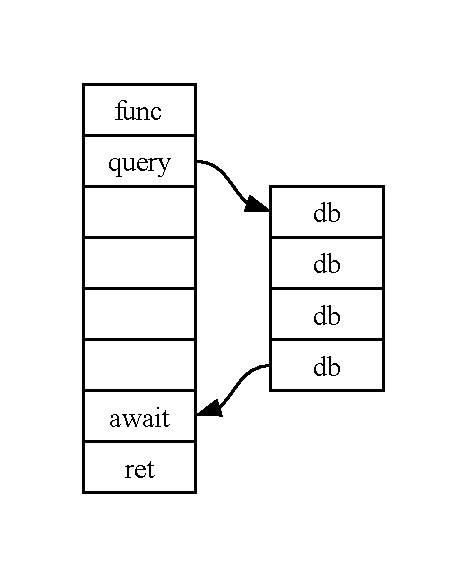
\includegraphics[width=\linewidth]{node_modules/@faaas/double-billing-problem/assets/double-billed-db.pdf}
    \caption{Double billing in action with call to persistent storage. Note that the function handler is idle whilst the DB is executing its query, yet still billed for the entire duration of the function.}
    \label{fig:double-billing-db}
\end{figure}

This is particularly problematic for serverless functions, which are designed to be stateless, and typically communicate with persistent storage to mainain state. This is further compounded by each function instance handling a single request at time.

In other less fine-grained systems such as CaaS, where a single instance handles multiple requests, this is not an issue, as the function can perform other useful work, such as accepting additional requests, while waiting for a response from an asynchronous service.

This issue also manifests more importantly when function invocations are nested as in Figure \ref{fig:double-billing-nested}. Considered an antipattern for this reason\cite{LambdaFunctionsCalling}, nested function invocations lead to a cascading effect of double billing, where each function invocation waits for the next to complete, and is billed for the entire duration of the called function.

\begin{figure}[t]
    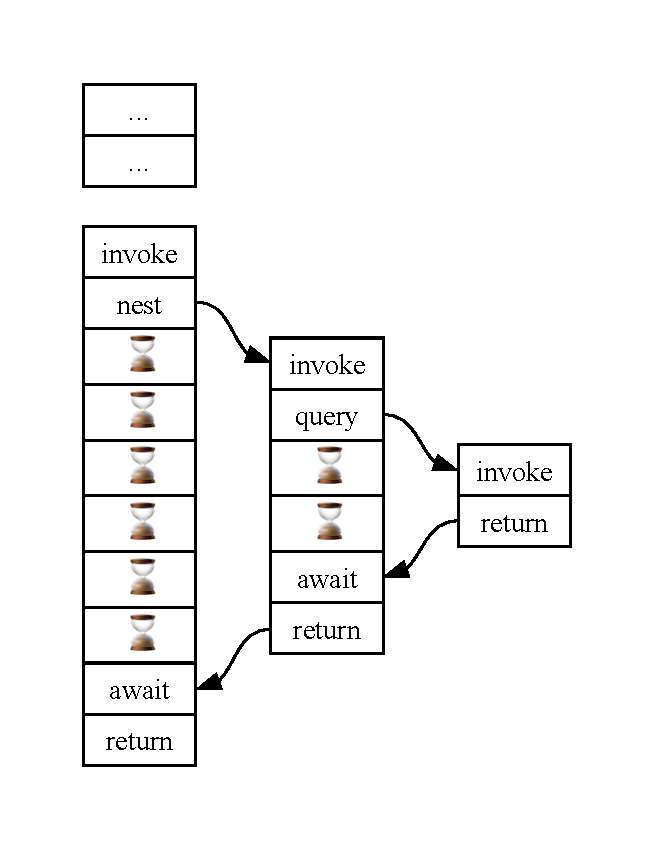
\includegraphics[width=\linewidth]{node_modules/@faaas/double-billing-problem/assets/double-billed-nested.pdf}
    \caption{Double billing in action with nested function invocations. Note that the function handler is idle whilst awaiting the nested invocation, yet still billed for the entire duration of the function.}
    \label{fig:double-billing-nested}
\end{figure}

\todo[inline]{Define CaaS}

\begin{figure*}[t]
    \begin{center}
        %% Creator: Matplotlib, PGF backend
%%
%% To include the figure in your LaTeX document, write
%%   \input{<filename>.pgf}
%%
%% Make sure the required packages are loaded in your preamble
%%   \usepackage{pgf}
%%
%% Also ensure that all the required font packages are loaded; for instance,
%% the lmodern package is sometimes necessary when using math font.
%%   \usepackage{lmodern}
%%
%% Figures using additional raster images can only be included by \input if
%% they are in the same directory as the main LaTeX file. For loading figures
%% from other directories you can use the `import` package
%%   \usepackage{import}
%%
%% and then include the figures with
%%   \import{<path to file>}{<filename>.pgf}
%%
%% Matplotlib used the following preamble
%%   \def\mathdefault#1{#1}
%%   \everymath=\expandafter{\the\everymath\displaystyle}
%%   
%%   \makeatletter\@ifpackageloaded{underscore}{}{\usepackage[strings]{underscore}}\makeatother
%%
\begingroup%
\makeatletter%
\begin{pgfpicture}%
\pgfpathrectangle{\pgfpointorigin}{\pgfqpoint{5.493059in}{3.854278in}}%
\pgfusepath{use as bounding box, clip}%
\begin{pgfscope}%
\pgfsetbuttcap%
\pgfsetmiterjoin%
\definecolor{currentfill}{rgb}{1.000000,1.000000,1.000000}%
\pgfsetfillcolor{currentfill}%
\pgfsetlinewidth{0.000000pt}%
\definecolor{currentstroke}{rgb}{1.000000,1.000000,1.000000}%
\pgfsetstrokecolor{currentstroke}%
\pgfsetdash{}{0pt}%
\pgfpathmoveto{\pgfqpoint{0.000000in}{0.000000in}}%
\pgfpathlineto{\pgfqpoint{5.493059in}{0.000000in}}%
\pgfpathlineto{\pgfqpoint{5.493059in}{3.854278in}}%
\pgfpathlineto{\pgfqpoint{0.000000in}{3.854278in}}%
\pgfpathlineto{\pgfqpoint{0.000000in}{0.000000in}}%
\pgfpathclose%
\pgfusepath{fill}%
\end{pgfscope}%
\begin{pgfscope}%
\pgfsetbuttcap%
\pgfsetmiterjoin%
\definecolor{currentfill}{rgb}{0.917647,0.917647,0.949020}%
\pgfsetfillcolor{currentfill}%
\pgfsetlinewidth{0.000000pt}%
\definecolor{currentstroke}{rgb}{0.000000,0.000000,0.000000}%
\pgfsetstrokecolor{currentstroke}%
\pgfsetstrokeopacity{0.000000}%
\pgfsetdash{}{0pt}%
\pgfpathmoveto{\pgfqpoint{0.800579in}{0.589352in}}%
\pgfpathlineto{\pgfqpoint{5.393059in}{0.589352in}}%
\pgfpathlineto{\pgfqpoint{5.393059in}{3.555205in}}%
\pgfpathlineto{\pgfqpoint{0.800579in}{3.555205in}}%
\pgfpathlineto{\pgfqpoint{0.800579in}{0.589352in}}%
\pgfpathclose%
\pgfusepath{fill}%
\end{pgfscope}%
\begin{pgfscope}%
\pgfpathrectangle{\pgfqpoint{0.800579in}{0.589352in}}{\pgfqpoint{4.592480in}{2.965853in}}%
\pgfusepath{clip}%
\pgfsetroundcap%
\pgfsetroundjoin%
\pgfsetlinewidth{1.003750pt}%
\definecolor{currentstroke}{rgb}{1.000000,1.000000,1.000000}%
\pgfsetstrokecolor{currentstroke}%
\pgfsetdash{}{0pt}%
\pgfpathmoveto{\pgfqpoint{1.009328in}{0.589352in}}%
\pgfpathlineto{\pgfqpoint{1.009328in}{3.555205in}}%
\pgfusepath{stroke}%
\end{pgfscope}%
\begin{pgfscope}%
\definecolor{textcolor}{rgb}{0.150000,0.150000,0.150000}%
\pgfsetstrokecolor{textcolor}%
\pgfsetfillcolor{textcolor}%
\pgftext[x=1.009328in,y=0.457407in,,top]{\color{textcolor}{\rmfamily\fontsize{11.000000}{13.200000}\selectfont\catcode`\^=\active\def^{\ifmmode\sp\else\^{}\fi}\catcode`\%=\active\def%{\%}$\mathdefault{2^{7}}$}}%
\end{pgfscope}%
\begin{pgfscope}%
\pgfpathrectangle{\pgfqpoint{0.800579in}{0.589352in}}{\pgfqpoint{4.592480in}{2.965853in}}%
\pgfusepath{clip}%
\pgfsetroundcap%
\pgfsetroundjoin%
\pgfsetlinewidth{1.003750pt}%
\definecolor{currentstroke}{rgb}{1.000000,1.000000,1.000000}%
\pgfsetstrokecolor{currentstroke}%
\pgfsetdash{}{0pt}%
\pgfpathmoveto{\pgfqpoint{2.053074in}{0.589352in}}%
\pgfpathlineto{\pgfqpoint{2.053074in}{3.555205in}}%
\pgfusepath{stroke}%
\end{pgfscope}%
\begin{pgfscope}%
\definecolor{textcolor}{rgb}{0.150000,0.150000,0.150000}%
\pgfsetstrokecolor{textcolor}%
\pgfsetfillcolor{textcolor}%
\pgftext[x=2.053074in,y=0.457407in,,top]{\color{textcolor}{\rmfamily\fontsize{11.000000}{13.200000}\selectfont\catcode`\^=\active\def^{\ifmmode\sp\else\^{}\fi}\catcode`\%=\active\def%{\%}$\mathdefault{2^{8}}$}}%
\end{pgfscope}%
\begin{pgfscope}%
\pgfpathrectangle{\pgfqpoint{0.800579in}{0.589352in}}{\pgfqpoint{4.592480in}{2.965853in}}%
\pgfusepath{clip}%
\pgfsetroundcap%
\pgfsetroundjoin%
\pgfsetlinewidth{1.003750pt}%
\definecolor{currentstroke}{rgb}{1.000000,1.000000,1.000000}%
\pgfsetstrokecolor{currentstroke}%
\pgfsetdash{}{0pt}%
\pgfpathmoveto{\pgfqpoint{3.096819in}{0.589352in}}%
\pgfpathlineto{\pgfqpoint{3.096819in}{3.555205in}}%
\pgfusepath{stroke}%
\end{pgfscope}%
\begin{pgfscope}%
\definecolor{textcolor}{rgb}{0.150000,0.150000,0.150000}%
\pgfsetstrokecolor{textcolor}%
\pgfsetfillcolor{textcolor}%
\pgftext[x=3.096819in,y=0.457407in,,top]{\color{textcolor}{\rmfamily\fontsize{11.000000}{13.200000}\selectfont\catcode`\^=\active\def^{\ifmmode\sp\else\^{}\fi}\catcode`\%=\active\def%{\%}$\mathdefault{2^{9}}$}}%
\end{pgfscope}%
\begin{pgfscope}%
\pgfpathrectangle{\pgfqpoint{0.800579in}{0.589352in}}{\pgfqpoint{4.592480in}{2.965853in}}%
\pgfusepath{clip}%
\pgfsetroundcap%
\pgfsetroundjoin%
\pgfsetlinewidth{1.003750pt}%
\definecolor{currentstroke}{rgb}{1.000000,1.000000,1.000000}%
\pgfsetstrokecolor{currentstroke}%
\pgfsetdash{}{0pt}%
\pgfpathmoveto{\pgfqpoint{4.140564in}{0.589352in}}%
\pgfpathlineto{\pgfqpoint{4.140564in}{3.555205in}}%
\pgfusepath{stroke}%
\end{pgfscope}%
\begin{pgfscope}%
\definecolor{textcolor}{rgb}{0.150000,0.150000,0.150000}%
\pgfsetstrokecolor{textcolor}%
\pgfsetfillcolor{textcolor}%
\pgftext[x=4.140564in,y=0.457407in,,top]{\color{textcolor}{\rmfamily\fontsize{11.000000}{13.200000}\selectfont\catcode`\^=\active\def^{\ifmmode\sp\else\^{}\fi}\catcode`\%=\active\def%{\%}$\mathdefault{2^{10}}$}}%
\end{pgfscope}%
\begin{pgfscope}%
\pgfpathrectangle{\pgfqpoint{0.800579in}{0.589352in}}{\pgfqpoint{4.592480in}{2.965853in}}%
\pgfusepath{clip}%
\pgfsetroundcap%
\pgfsetroundjoin%
\pgfsetlinewidth{1.003750pt}%
\definecolor{currentstroke}{rgb}{1.000000,1.000000,1.000000}%
\pgfsetstrokecolor{currentstroke}%
\pgfsetdash{}{0pt}%
\pgfpathmoveto{\pgfqpoint{5.184310in}{0.589352in}}%
\pgfpathlineto{\pgfqpoint{5.184310in}{3.555205in}}%
\pgfusepath{stroke}%
\end{pgfscope}%
\begin{pgfscope}%
\definecolor{textcolor}{rgb}{0.150000,0.150000,0.150000}%
\pgfsetstrokecolor{textcolor}%
\pgfsetfillcolor{textcolor}%
\pgftext[x=5.184310in,y=0.457407in,,top]{\color{textcolor}{\rmfamily\fontsize{11.000000}{13.200000}\selectfont\catcode`\^=\active\def^{\ifmmode\sp\else\^{}\fi}\catcode`\%=\active\def%{\%}$\mathdefault{2^{11}}$}}%
\end{pgfscope}%
\begin{pgfscope}%
\definecolor{textcolor}{rgb}{0.150000,0.150000,0.150000}%
\pgfsetstrokecolor{textcolor}%
\pgfsetfillcolor{textcolor}%
\pgftext[x=3.096819in,y=0.266667in,,top]{\color{textcolor}{\rmfamily\fontsize{12.000000}{14.400000}\selectfont\catcode`\^=\active\def^{\ifmmode\sp\else\^{}\fi}\catcode`\%=\active\def%{\%}Memory (MB)}}%
\end{pgfscope}%
\begin{pgfscope}%
\pgfpathrectangle{\pgfqpoint{0.800579in}{0.589352in}}{\pgfqpoint{4.592480in}{2.965853in}}%
\pgfusepath{clip}%
\pgfsetroundcap%
\pgfsetroundjoin%
\pgfsetlinewidth{1.003750pt}%
\definecolor{currentstroke}{rgb}{1.000000,1.000000,1.000000}%
\pgfsetstrokecolor{currentstroke}%
\pgfsetdash{}{0pt}%
\pgfpathmoveto{\pgfqpoint{0.800579in}{0.627869in}}%
\pgfpathlineto{\pgfqpoint{5.393059in}{0.627869in}}%
\pgfusepath{stroke}%
\end{pgfscope}%
\begin{pgfscope}%
\definecolor{textcolor}{rgb}{0.150000,0.150000,0.150000}%
\pgfsetstrokecolor{textcolor}%
\pgfsetfillcolor{textcolor}%
\pgftext[x=0.322222in, y=0.575063in, left, base]{\color{textcolor}{\rmfamily\fontsize{11.000000}{13.200000}\selectfont\catcode`\^=\active\def^{\ifmmode\sp\else\^{}\fi}\catcode`\%=\active\def%{\%}$\mathdefault{0.000}$}}%
\end{pgfscope}%
\begin{pgfscope}%
\pgfpathrectangle{\pgfqpoint{0.800579in}{0.589352in}}{\pgfqpoint{4.592480in}{2.965853in}}%
\pgfusepath{clip}%
\pgfsetroundcap%
\pgfsetroundjoin%
\pgfsetlinewidth{1.003750pt}%
\definecolor{currentstroke}{rgb}{1.000000,1.000000,1.000000}%
\pgfsetstrokecolor{currentstroke}%
\pgfsetdash{}{0pt}%
\pgfpathmoveto{\pgfqpoint{0.800579in}{1.029094in}}%
\pgfpathlineto{\pgfqpoint{5.393059in}{1.029094in}}%
\pgfusepath{stroke}%
\end{pgfscope}%
\begin{pgfscope}%
\definecolor{textcolor}{rgb}{0.150000,0.150000,0.150000}%
\pgfsetstrokecolor{textcolor}%
\pgfsetfillcolor{textcolor}%
\pgftext[x=0.322222in, y=0.976287in, left, base]{\color{textcolor}{\rmfamily\fontsize{11.000000}{13.200000}\selectfont\catcode`\^=\active\def^{\ifmmode\sp\else\^{}\fi}\catcode`\%=\active\def%{\%}$\mathdefault{0.025}$}}%
\end{pgfscope}%
\begin{pgfscope}%
\pgfpathrectangle{\pgfqpoint{0.800579in}{0.589352in}}{\pgfqpoint{4.592480in}{2.965853in}}%
\pgfusepath{clip}%
\pgfsetroundcap%
\pgfsetroundjoin%
\pgfsetlinewidth{1.003750pt}%
\definecolor{currentstroke}{rgb}{1.000000,1.000000,1.000000}%
\pgfsetstrokecolor{currentstroke}%
\pgfsetdash{}{0pt}%
\pgfpathmoveto{\pgfqpoint{0.800579in}{1.430319in}}%
\pgfpathlineto{\pgfqpoint{5.393059in}{1.430319in}}%
\pgfusepath{stroke}%
\end{pgfscope}%
\begin{pgfscope}%
\definecolor{textcolor}{rgb}{0.150000,0.150000,0.150000}%
\pgfsetstrokecolor{textcolor}%
\pgfsetfillcolor{textcolor}%
\pgftext[x=0.322222in, y=1.377512in, left, base]{\color{textcolor}{\rmfamily\fontsize{11.000000}{13.200000}\selectfont\catcode`\^=\active\def^{\ifmmode\sp\else\^{}\fi}\catcode`\%=\active\def%{\%}$\mathdefault{0.050}$}}%
\end{pgfscope}%
\begin{pgfscope}%
\pgfpathrectangle{\pgfqpoint{0.800579in}{0.589352in}}{\pgfqpoint{4.592480in}{2.965853in}}%
\pgfusepath{clip}%
\pgfsetroundcap%
\pgfsetroundjoin%
\pgfsetlinewidth{1.003750pt}%
\definecolor{currentstroke}{rgb}{1.000000,1.000000,1.000000}%
\pgfsetstrokecolor{currentstroke}%
\pgfsetdash{}{0pt}%
\pgfpathmoveto{\pgfqpoint{0.800579in}{1.831543in}}%
\pgfpathlineto{\pgfqpoint{5.393059in}{1.831543in}}%
\pgfusepath{stroke}%
\end{pgfscope}%
\begin{pgfscope}%
\definecolor{textcolor}{rgb}{0.150000,0.150000,0.150000}%
\pgfsetstrokecolor{textcolor}%
\pgfsetfillcolor{textcolor}%
\pgftext[x=0.322222in, y=1.778737in, left, base]{\color{textcolor}{\rmfamily\fontsize{11.000000}{13.200000}\selectfont\catcode`\^=\active\def^{\ifmmode\sp\else\^{}\fi}\catcode`\%=\active\def%{\%}$\mathdefault{0.075}$}}%
\end{pgfscope}%
\begin{pgfscope}%
\pgfpathrectangle{\pgfqpoint{0.800579in}{0.589352in}}{\pgfqpoint{4.592480in}{2.965853in}}%
\pgfusepath{clip}%
\pgfsetroundcap%
\pgfsetroundjoin%
\pgfsetlinewidth{1.003750pt}%
\definecolor{currentstroke}{rgb}{1.000000,1.000000,1.000000}%
\pgfsetstrokecolor{currentstroke}%
\pgfsetdash{}{0pt}%
\pgfpathmoveto{\pgfqpoint{0.800579in}{2.232768in}}%
\pgfpathlineto{\pgfqpoint{5.393059in}{2.232768in}}%
\pgfusepath{stroke}%
\end{pgfscope}%
\begin{pgfscope}%
\definecolor{textcolor}{rgb}{0.150000,0.150000,0.150000}%
\pgfsetstrokecolor{textcolor}%
\pgfsetfillcolor{textcolor}%
\pgftext[x=0.322222in, y=2.179961in, left, base]{\color{textcolor}{\rmfamily\fontsize{11.000000}{13.200000}\selectfont\catcode`\^=\active\def^{\ifmmode\sp\else\^{}\fi}\catcode`\%=\active\def%{\%}$\mathdefault{0.100}$}}%
\end{pgfscope}%
\begin{pgfscope}%
\pgfpathrectangle{\pgfqpoint{0.800579in}{0.589352in}}{\pgfqpoint{4.592480in}{2.965853in}}%
\pgfusepath{clip}%
\pgfsetroundcap%
\pgfsetroundjoin%
\pgfsetlinewidth{1.003750pt}%
\definecolor{currentstroke}{rgb}{1.000000,1.000000,1.000000}%
\pgfsetstrokecolor{currentstroke}%
\pgfsetdash{}{0pt}%
\pgfpathmoveto{\pgfqpoint{0.800579in}{2.633993in}}%
\pgfpathlineto{\pgfqpoint{5.393059in}{2.633993in}}%
\pgfusepath{stroke}%
\end{pgfscope}%
\begin{pgfscope}%
\definecolor{textcolor}{rgb}{0.150000,0.150000,0.150000}%
\pgfsetstrokecolor{textcolor}%
\pgfsetfillcolor{textcolor}%
\pgftext[x=0.322222in, y=2.581186in, left, base]{\color{textcolor}{\rmfamily\fontsize{11.000000}{13.200000}\selectfont\catcode`\^=\active\def^{\ifmmode\sp\else\^{}\fi}\catcode`\%=\active\def%{\%}$\mathdefault{0.125}$}}%
\end{pgfscope}%
\begin{pgfscope}%
\pgfpathrectangle{\pgfqpoint{0.800579in}{0.589352in}}{\pgfqpoint{4.592480in}{2.965853in}}%
\pgfusepath{clip}%
\pgfsetroundcap%
\pgfsetroundjoin%
\pgfsetlinewidth{1.003750pt}%
\definecolor{currentstroke}{rgb}{1.000000,1.000000,1.000000}%
\pgfsetstrokecolor{currentstroke}%
\pgfsetdash{}{0pt}%
\pgfpathmoveto{\pgfqpoint{0.800579in}{3.035218in}}%
\pgfpathlineto{\pgfqpoint{5.393059in}{3.035218in}}%
\pgfusepath{stroke}%
\end{pgfscope}%
\begin{pgfscope}%
\definecolor{textcolor}{rgb}{0.150000,0.150000,0.150000}%
\pgfsetstrokecolor{textcolor}%
\pgfsetfillcolor{textcolor}%
\pgftext[x=0.322222in, y=2.982411in, left, base]{\color{textcolor}{\rmfamily\fontsize{11.000000}{13.200000}\selectfont\catcode`\^=\active\def^{\ifmmode\sp\else\^{}\fi}\catcode`\%=\active\def%{\%}$\mathdefault{0.150}$}}%
\end{pgfscope}%
\begin{pgfscope}%
\pgfpathrectangle{\pgfqpoint{0.800579in}{0.589352in}}{\pgfqpoint{4.592480in}{2.965853in}}%
\pgfusepath{clip}%
\pgfsetroundcap%
\pgfsetroundjoin%
\pgfsetlinewidth{1.003750pt}%
\definecolor{currentstroke}{rgb}{1.000000,1.000000,1.000000}%
\pgfsetstrokecolor{currentstroke}%
\pgfsetdash{}{0pt}%
\pgfpathmoveto{\pgfqpoint{0.800579in}{3.436442in}}%
\pgfpathlineto{\pgfqpoint{5.393059in}{3.436442in}}%
\pgfusepath{stroke}%
\end{pgfscope}%
\begin{pgfscope}%
\definecolor{textcolor}{rgb}{0.150000,0.150000,0.150000}%
\pgfsetstrokecolor{textcolor}%
\pgfsetfillcolor{textcolor}%
\pgftext[x=0.322222in, y=3.383636in, left, base]{\color{textcolor}{\rmfamily\fontsize{11.000000}{13.200000}\selectfont\catcode`\^=\active\def^{\ifmmode\sp\else\^{}\fi}\catcode`\%=\active\def%{\%}$\mathdefault{0.175}$}}%
\end{pgfscope}%
\begin{pgfscope}%
\definecolor{textcolor}{rgb}{0.150000,0.150000,0.150000}%
\pgfsetstrokecolor{textcolor}%
\pgfsetfillcolor{textcolor}%
\pgftext[x=0.266667in,y=2.072278in,,bottom,rotate=90.000000]{\color{textcolor}{\rmfamily\fontsize{12.000000}{14.400000}\selectfont\catcode`\^=\active\def^{\ifmmode\sp\else\^{}\fi}\catcode`\%=\active\def%{\%}Yield time (s)}}%
\end{pgfscope}%
\begin{pgfscope}%
\pgfpathrectangle{\pgfqpoint{0.800579in}{0.589352in}}{\pgfqpoint{4.592480in}{2.965853in}}%
\pgfusepath{clip}%
\pgfsetbuttcap%
\pgfsetmiterjoin%
\definecolor{currentfill}{rgb}{0.768627,0.305882,0.321569}%
\pgfsetfillcolor{currentfill}%
\pgfsetfillopacity{0.200000}%
\pgfsetlinewidth{1.003750pt}%
\definecolor{currentstroke}{rgb}{0.768627,0.305882,0.321569}%
\pgfsetstrokecolor{currentstroke}%
\pgfsetstrokeopacity{0.200000}%
\pgfsetdash{}{0pt}%
\pgfpathmoveto{\pgfqpoint{0.800579in}{1.590809in}}%
\pgfpathlineto{\pgfqpoint{0.800579in}{2.072278in}}%
\pgfpathlineto{\pgfqpoint{5.393059in}{2.072278in}}%
\pgfpathlineto{\pgfqpoint{5.393059in}{1.590809in}}%
\pgfpathlineto{\pgfqpoint{0.800579in}{1.590809in}}%
\pgfpathclose%
\pgfusepath{stroke,fill}%
\end{pgfscope}%
\begin{pgfscope}%
\pgfpathrectangle{\pgfqpoint{0.800579in}{0.589352in}}{\pgfqpoint{4.592480in}{2.965853in}}%
\pgfusepath{clip}%
\pgfsetbuttcap%
\pgfsetmiterjoin%
\definecolor{currentfill}{rgb}{0.298039,0.447059,0.690196}%
\pgfsetfillcolor{currentfill}%
\pgfsetfillopacity{0.200000}%
\pgfsetlinewidth{1.003750pt}%
\definecolor{currentstroke}{rgb}{0.298039,0.447059,0.690196}%
\pgfsetstrokecolor{currentstroke}%
\pgfsetstrokeopacity{0.200000}%
\pgfsetdash{}{0pt}%
\pgfpathmoveto{\pgfqpoint{0.800579in}{0.788359in}}%
\pgfpathlineto{\pgfqpoint{0.800579in}{1.029094in}}%
\pgfpathlineto{\pgfqpoint{5.393059in}{1.029094in}}%
\pgfpathlineto{\pgfqpoint{5.393059in}{0.788359in}}%
\pgfpathlineto{\pgfqpoint{0.800579in}{0.788359in}}%
\pgfpathclose%
\pgfusepath{stroke,fill}%
\end{pgfscope}%
\begin{pgfscope}%
\pgfpathrectangle{\pgfqpoint{0.800579in}{0.589352in}}{\pgfqpoint{4.592480in}{2.965853in}}%
\pgfusepath{clip}%
\pgfsetroundcap%
\pgfsetroundjoin%
\pgfsetlinewidth{1.505625pt}%
\definecolor{currentstroke}{rgb}{0.298039,0.447059,0.690196}%
\pgfsetstrokecolor{currentstroke}%
\pgfsetdash{}{0pt}%
\pgfpathmoveto{\pgfqpoint{1.009328in}{2.168572in}}%
\pgfpathlineto{\pgfqpoint{1.021047in}{2.168572in}}%
\pgfpathlineto{\pgfqpoint{1.044213in}{2.136474in}}%
\pgfpathlineto{\pgfqpoint{1.055664in}{2.136474in}}%
\pgfpathlineto{\pgfqpoint{1.078309in}{2.104376in}}%
\pgfpathlineto{\pgfqpoint{1.089504in}{2.104376in}}%
\pgfpathlineto{\pgfqpoint{1.111649in}{2.072278in}}%
\pgfpathlineto{\pgfqpoint{1.122600in}{2.072278in}}%
\pgfpathlineto{\pgfqpoint{1.144267in}{2.040180in}}%
\pgfpathlineto{\pgfqpoint{1.154984in}{2.040180in}}%
\pgfpathlineto{\pgfqpoint{1.176193in}{2.008082in}}%
\pgfpathlineto{\pgfqpoint{1.186687in}{2.008082in}}%
\pgfpathlineto{\pgfqpoint{1.197108in}{1.992033in}}%
\pgfpathlineto{\pgfqpoint{1.207457in}{1.992033in}}%
\pgfpathlineto{\pgfqpoint{1.217735in}{1.975984in}}%
\pgfpathlineto{\pgfqpoint{1.227944in}{1.975984in}}%
\pgfpathlineto{\pgfqpoint{1.248157in}{1.943886in}}%
\pgfpathlineto{\pgfqpoint{1.258162in}{1.943886in}}%
\pgfpathlineto{\pgfqpoint{1.268101in}{1.927837in}}%
\pgfpathlineto{\pgfqpoint{1.277976in}{1.927837in}}%
\pgfpathlineto{\pgfqpoint{1.287785in}{1.911788in}}%
\pgfpathlineto{\pgfqpoint{1.297532in}{1.911788in}}%
\pgfpathlineto{\pgfqpoint{1.307215in}{1.895739in}}%
\pgfpathlineto{\pgfqpoint{1.316837in}{1.895739in}}%
\pgfpathlineto{\pgfqpoint{1.326398in}{1.879690in}}%
\pgfpathlineto{\pgfqpoint{1.335898in}{1.879690in}}%
\pgfpathlineto{\pgfqpoint{1.345339in}{1.863641in}}%
\pgfpathlineto{\pgfqpoint{1.354721in}{1.863641in}}%
\pgfpathlineto{\pgfqpoint{1.364045in}{1.847592in}}%
\pgfpathlineto{\pgfqpoint{1.373312in}{1.847592in}}%
\pgfpathlineto{\pgfqpoint{1.382521in}{1.831543in}}%
\pgfpathlineto{\pgfqpoint{1.400774in}{1.831543in}}%
\pgfpathlineto{\pgfqpoint{1.409818in}{1.815494in}}%
\pgfpathlineto{\pgfqpoint{1.418808in}{1.815494in}}%
\pgfpathlineto{\pgfqpoint{1.427744in}{1.799445in}}%
\pgfpathlineto{\pgfqpoint{1.436628in}{1.799445in}}%
\pgfpathlineto{\pgfqpoint{1.445460in}{1.783396in}}%
\pgfpathlineto{\pgfqpoint{1.462969in}{1.783396in}}%
\pgfpathlineto{\pgfqpoint{1.471648in}{1.767347in}}%
\pgfpathlineto{\pgfqpoint{1.480278in}{1.767347in}}%
\pgfpathlineto{\pgfqpoint{1.488858in}{1.751299in}}%
\pgfpathlineto{\pgfqpoint{1.505873in}{1.751299in}}%
\pgfpathlineto{\pgfqpoint{1.514309in}{1.735250in}}%
\pgfpathlineto{\pgfqpoint{1.522698in}{1.735250in}}%
\pgfpathlineto{\pgfqpoint{1.531040in}{1.719201in}}%
\pgfpathlineto{\pgfqpoint{1.547588in}{1.719201in}}%
\pgfpathlineto{\pgfqpoint{1.555794in}{1.703152in}}%
\pgfpathlineto{\pgfqpoint{1.572073in}{1.703152in}}%
\pgfpathlineto{\pgfqpoint{1.580147in}{1.687103in}}%
\pgfpathlineto{\pgfqpoint{1.596166in}{1.687103in}}%
\pgfpathlineto{\pgfqpoint{1.604112in}{1.671054in}}%
\pgfpathlineto{\pgfqpoint{1.612017in}{1.671054in}}%
\pgfpathlineto{\pgfqpoint{1.619880in}{1.655005in}}%
\pgfpathlineto{\pgfqpoint{1.643226in}{1.655005in}}%
\pgfpathlineto{\pgfqpoint{1.650929in}{1.638956in}}%
\pgfpathlineto{\pgfqpoint{1.666216in}{1.638956in}}%
\pgfpathlineto{\pgfqpoint{1.673802in}{1.622907in}}%
\pgfpathlineto{\pgfqpoint{1.688860in}{1.622907in}}%
\pgfpathlineto{\pgfqpoint{1.696333in}{1.606858in}}%
\pgfpathlineto{\pgfqpoint{1.711169in}{1.606858in}}%
\pgfpathlineto{\pgfqpoint{1.718532in}{1.590809in}}%
\pgfpathlineto{\pgfqpoint{1.740409in}{1.590809in}}%
\pgfpathlineto{\pgfqpoint{1.747631in}{1.574760in}}%
\pgfpathlineto{\pgfqpoint{1.761972in}{1.574760in}}%
\pgfpathlineto{\pgfqpoint{1.769092in}{1.558711in}}%
\pgfpathlineto{\pgfqpoint{1.790251in}{1.558711in}}%
\pgfpathlineto{\pgfqpoint{1.797239in}{1.542662in}}%
\pgfpathlineto{\pgfqpoint{1.818009in}{1.542662in}}%
\pgfpathlineto{\pgfqpoint{1.824869in}{1.526613in}}%
\pgfpathlineto{\pgfqpoint{1.845264in}{1.526613in}}%
\pgfpathlineto{\pgfqpoint{1.852001in}{1.510564in}}%
\pgfpathlineto{\pgfqpoint{1.872034in}{1.510564in}}%
\pgfpathlineto{\pgfqpoint{1.878653in}{1.494515in}}%
\pgfpathlineto{\pgfqpoint{1.898337in}{1.494515in}}%
\pgfpathlineto{\pgfqpoint{1.904842in}{1.478466in}}%
\pgfpathlineto{\pgfqpoint{1.930583in}{1.478466in}}%
\pgfpathlineto{\pgfqpoint{1.936950in}{1.462417in}}%
\pgfpathlineto{\pgfqpoint{1.955891in}{1.462417in}}%
\pgfpathlineto{\pgfqpoint{1.962152in}{1.446368in}}%
\pgfpathlineto{\pgfqpoint{1.986940in}{1.446368in}}%
\pgfpathlineto{\pgfqpoint{1.993073in}{1.430319in}}%
\pgfpathlineto{\pgfqpoint{2.017361in}{1.430319in}}%
\pgfpathlineto{\pgfqpoint{2.023372in}{1.414270in}}%
\pgfpathlineto{\pgfqpoint{2.047180in}{1.414270in}}%
\pgfpathlineto{\pgfqpoint{2.053074in}{1.398221in}}%
\pgfpathlineto{\pgfqpoint{2.082200in}{1.398221in}}%
\pgfpathlineto{\pgfqpoint{2.087959in}{1.382172in}}%
\pgfpathlineto{\pgfqpoint{2.116425in}{1.382172in}}%
\pgfpathlineto{\pgfqpoint{2.122054in}{1.366123in}}%
\pgfpathlineto{\pgfqpoint{2.149888in}{1.366123in}}%
\pgfpathlineto{\pgfqpoint{2.155394in}{1.350074in}}%
\pgfpathlineto{\pgfqpoint{2.182625in}{1.350074in}}%
\pgfpathlineto{\pgfqpoint{2.188012in}{1.334025in}}%
\pgfpathlineto{\pgfqpoint{2.214664in}{1.334025in}}%
\pgfpathlineto{\pgfqpoint{2.219939in}{1.317976in}}%
\pgfpathlineto{\pgfqpoint{2.251202in}{1.317976in}}%
\pgfpathlineto{\pgfqpoint{2.256350in}{1.301927in}}%
\pgfpathlineto{\pgfqpoint{2.286874in}{1.301927in}}%
\pgfpathlineto{\pgfqpoint{2.291902in}{1.285878in}}%
\pgfpathlineto{\pgfqpoint{2.326634in}{1.285878in}}%
\pgfpathlineto{\pgfqpoint{2.331531in}{1.269829in}}%
\pgfpathlineto{\pgfqpoint{2.365371in}{1.269829in}}%
\pgfpathlineto{\pgfqpoint{2.370143in}{1.253780in}}%
\pgfpathlineto{\pgfqpoint{2.403136in}{1.253780in}}%
\pgfpathlineto{\pgfqpoint{2.407790in}{1.237731in}}%
\pgfpathlineto{\pgfqpoint{2.444519in}{1.237731in}}%
\pgfpathlineto{\pgfqpoint{2.449048in}{1.221682in}}%
\pgfpathlineto{\pgfqpoint{2.484796in}{1.221682in}}%
\pgfpathlineto{\pgfqpoint{2.489205in}{1.205633in}}%
\pgfpathlineto{\pgfqpoint{2.528319in}{1.205633in}}%
\pgfpathlineto{\pgfqpoint{2.532603in}{1.189584in}}%
\pgfpathlineto{\pgfqpoint{2.570620in}{1.189584in}}%
\pgfpathlineto{\pgfqpoint{2.574785in}{1.173535in}}%
\pgfpathlineto{\pgfqpoint{2.615818in}{1.173535in}}%
\pgfpathlineto{\pgfqpoint{2.619861in}{1.157486in}}%
\pgfpathlineto{\pgfqpoint{2.659699in}{1.157486in}}%
\pgfpathlineto{\pgfqpoint{2.663625in}{1.141437in}}%
\pgfpathlineto{\pgfqpoint{2.709962in}{1.141437in}}%
\pgfpathlineto{\pgfqpoint{2.713759in}{1.125388in}}%
\pgfpathlineto{\pgfqpoint{2.758601in}{1.125388in}}%
\pgfpathlineto{\pgfqpoint{2.762278in}{1.109339in}}%
\pgfpathlineto{\pgfqpoint{2.809282in}{1.109339in}}%
\pgfpathlineto{\pgfqpoint{2.812837in}{1.093290in}}%
\pgfpathlineto{\pgfqpoint{2.861754in}{1.093290in}}%
\pgfpathlineto{\pgfqpoint{2.865188in}{1.077241in}}%
\pgfpathlineto{\pgfqpoint{2.919093in}{1.077241in}}%
\pgfpathlineto{\pgfqpoint{2.922399in}{1.061192in}}%
\pgfpathlineto{\pgfqpoint{2.974328in}{1.061192in}}%
\pgfpathlineto{\pgfqpoint{2.977515in}{1.045143in}}%
\pgfpathlineto{\pgfqpoint{3.033755in}{1.045143in}}%
\pgfpathlineto{\pgfqpoint{3.036819in}{1.029094in}}%
\pgfpathlineto{\pgfqpoint{3.093875in}{1.029094in}}%
\pgfpathlineto{\pgfqpoint{3.096819in}{1.013045in}}%
\pgfpathlineto{\pgfqpoint{3.160170in}{1.013045in}}%
\pgfpathlineto{\pgfqpoint{3.162987in}{0.996996in}}%
\pgfpathlineto{\pgfqpoint{3.226370in}{0.996996in}}%
\pgfpathlineto{\pgfqpoint{3.229066in}{0.980947in}}%
\pgfpathlineto{\pgfqpoint{3.297524in}{0.980947in}}%
\pgfpathlineto{\pgfqpoint{3.300095in}{0.964898in}}%
\pgfpathlineto{\pgfqpoint{3.370379in}{0.964898in}}%
\pgfpathlineto{\pgfqpoint{3.372830in}{0.948849in}}%
\pgfpathlineto{\pgfqpoint{3.446881in}{0.948849in}}%
\pgfpathlineto{\pgfqpoint{3.449210in}{0.932800in}}%
\pgfpathlineto{\pgfqpoint{3.528541in}{0.932800in}}%
\pgfpathlineto{\pgfqpoint{3.530747in}{0.916751in}}%
\pgfpathlineto{\pgfqpoint{3.614365in}{0.916751in}}%
\pgfpathlineto{\pgfqpoint{3.616449in}{0.900702in}}%
\pgfpathlineto{\pgfqpoint{3.705409in}{0.900702in}}%
\pgfpathlineto{\pgfqpoint{3.707371in}{0.884653in}}%
\pgfpathlineto{\pgfqpoint{3.804186in}{0.884653in}}%
\pgfpathlineto{\pgfqpoint{3.806023in}{0.868604in}}%
\pgfpathlineto{\pgfqpoint{3.907217in}{0.868604in}}%
\pgfpathlineto{\pgfqpoint{3.908933in}{0.852555in}}%
\pgfpathlineto{\pgfqpoint{4.019668in}{0.852555in}}%
\pgfpathlineto{\pgfqpoint{4.021260in}{0.836506in}}%
\pgfpathlineto{\pgfqpoint{4.139093in}{0.836506in}}%
\pgfpathlineto{\pgfqpoint{4.140564in}{0.820457in}}%
\pgfpathlineto{\pgfqpoint{4.271464in}{0.820457in}}%
\pgfpathlineto{\pgfqpoint{4.272811in}{0.804408in}}%
\pgfpathlineto{\pgfqpoint{4.414125in}{0.804408in}}%
\pgfpathlineto{\pgfqpoint{4.415350in}{0.788359in}}%
\pgfpathlineto{\pgfqpoint{4.573390in}{0.788359in}}%
\pgfpathlineto{\pgfqpoint{4.575595in}{0.772310in}}%
\pgfpathlineto{\pgfqpoint{4.750135in}{0.772310in}}%
\pgfpathlineto{\pgfqpoint{4.752096in}{0.756261in}}%
\pgfpathlineto{\pgfqpoint{4.951821in}{0.756261in}}%
\pgfpathlineto{\pgfqpoint{4.953536in}{0.740212in}}%
\pgfpathlineto{\pgfqpoint{5.183574in}{0.740212in}}%
\pgfpathlineto{\pgfqpoint{5.184310in}{0.724163in}}%
\pgfpathlineto{\pgfqpoint{5.184310in}{0.724163in}}%
\pgfusepath{stroke}%
\end{pgfscope}%
\begin{pgfscope}%
\pgfpathrectangle{\pgfqpoint{0.800579in}{0.589352in}}{\pgfqpoint{4.592480in}{2.965853in}}%
\pgfusepath{clip}%
\pgfsetroundcap%
\pgfsetroundjoin%
\pgfsetlinewidth{1.505625pt}%
\definecolor{currentstroke}{rgb}{0.866667,0.517647,0.321569}%
\pgfsetstrokecolor{currentstroke}%
\pgfsetdash{}{0pt}%
\pgfpathmoveto{\pgfqpoint{1.009328in}{2.232768in}}%
\pgfpathlineto{\pgfqpoint{2.047180in}{2.232768in}}%
\pgfpathlineto{\pgfqpoint{2.053074in}{1.430319in}}%
\pgfpathlineto{\pgfqpoint{2.659699in}{1.430319in}}%
\pgfpathlineto{\pgfqpoint{2.663625in}{1.173535in}}%
\pgfpathlineto{\pgfqpoint{3.093875in}{1.173535in}}%
\pgfpathlineto{\pgfqpoint{3.096819in}{1.029094in}}%
\pgfpathlineto{\pgfqpoint{3.430475in}{1.029094in}}%
\pgfpathlineto{\pgfqpoint{3.432830in}{0.948849in}}%
\pgfpathlineto{\pgfqpoint{3.705409in}{0.948849in}}%
\pgfpathlineto{\pgfqpoint{3.707371in}{0.900702in}}%
\pgfpathlineto{\pgfqpoint{3.937810in}{0.900702in}}%
\pgfpathlineto{\pgfqpoint{3.939492in}{0.868604in}}%
\pgfpathlineto{\pgfqpoint{4.139093in}{0.868604in}}%
\pgfpathlineto{\pgfqpoint{4.140564in}{0.836506in}}%
\pgfpathlineto{\pgfqpoint{4.316615in}{0.836506in}}%
\pgfpathlineto{\pgfqpoint{4.317923in}{0.820457in}}%
\pgfpathlineto{\pgfqpoint{4.475398in}{0.820457in}}%
\pgfpathlineto{\pgfqpoint{4.476575in}{0.788359in}}%
\pgfpathlineto{\pgfqpoint{4.750135in}{0.788359in}}%
\pgfpathlineto{\pgfqpoint{4.752096in}{0.772310in}}%
\pgfpathlineto{\pgfqpoint{5.184310in}{0.772310in}}%
\pgfpathlineto{\pgfqpoint{5.184310in}{0.772310in}}%
\pgfusepath{stroke}%
\end{pgfscope}%
\begin{pgfscope}%
\pgfpathrectangle{\pgfqpoint{0.800579in}{0.589352in}}{\pgfqpoint{4.592480in}{2.965853in}}%
\pgfusepath{clip}%
\pgfsetroundcap%
\pgfsetroundjoin%
\pgfsetlinewidth{1.505625pt}%
\definecolor{currentstroke}{rgb}{0.333333,0.658824,0.407843}%
\pgfsetstrokecolor{currentstroke}%
\pgfsetdash{}{0pt}%
\pgfpathmoveto{\pgfqpoint{1.009328in}{3.420393in}}%
\pgfpathlineto{\pgfqpoint{2.047180in}{3.420393in}}%
\pgfpathlineto{\pgfqpoint{2.053074in}{2.024131in}}%
\pgfpathlineto{\pgfqpoint{3.093875in}{2.024131in}}%
\pgfpathlineto{\pgfqpoint{3.096819in}{1.334025in}}%
\pgfpathlineto{\pgfqpoint{4.139093in}{1.334025in}}%
\pgfpathlineto{\pgfqpoint{4.140564in}{1.029094in}}%
\pgfpathlineto{\pgfqpoint{5.183574in}{1.029094in}}%
\pgfpathlineto{\pgfqpoint{5.184310in}{0.852555in}}%
\pgfpathlineto{\pgfqpoint{5.184310in}{0.852555in}}%
\pgfusepath{stroke}%
\end{pgfscope}%
\begin{pgfscope}%
\pgfpathrectangle{\pgfqpoint{0.800579in}{0.589352in}}{\pgfqpoint{4.592480in}{2.965853in}}%
\pgfusepath{clip}%
\pgfsetbuttcap%
\pgfsetroundjoin%
\pgfsetlinewidth{1.505625pt}%
\definecolor{currentstroke}{rgb}{0.768627,0.305882,0.321569}%
\pgfsetstrokecolor{currentstroke}%
\pgfsetstrokeopacity{0.200000}%
\pgfsetdash{{5.550000pt}{2.400000pt}}{0.000000pt}%
\pgfpathmoveto{\pgfqpoint{0.800579in}{2.072278in}}%
\pgfpathlineto{\pgfqpoint{5.393059in}{2.072278in}}%
\pgfusepath{stroke}%
\end{pgfscope}%
\begin{pgfscope}%
\pgfpathrectangle{\pgfqpoint{0.800579in}{0.589352in}}{\pgfqpoint{4.592480in}{2.965853in}}%
\pgfusepath{clip}%
\pgfsetbuttcap%
\pgfsetroundjoin%
\pgfsetlinewidth{1.505625pt}%
\definecolor{currentstroke}{rgb}{0.768627,0.305882,0.321569}%
\pgfsetstrokecolor{currentstroke}%
\pgfsetstrokeopacity{0.200000}%
\pgfsetdash{{5.550000pt}{2.400000pt}}{0.000000pt}%
\pgfpathmoveto{\pgfqpoint{0.800579in}{1.590809in}}%
\pgfpathlineto{\pgfqpoint{5.393059in}{1.590809in}}%
\pgfusepath{stroke}%
\end{pgfscope}%
\begin{pgfscope}%
\pgfpathrectangle{\pgfqpoint{0.800579in}{0.589352in}}{\pgfqpoint{4.592480in}{2.965853in}}%
\pgfusepath{clip}%
\pgfsetbuttcap%
\pgfsetroundjoin%
\pgfsetlinewidth{1.505625pt}%
\definecolor{currentstroke}{rgb}{0.298039,0.447059,0.690196}%
\pgfsetstrokecolor{currentstroke}%
\pgfsetstrokeopacity{0.200000}%
\pgfsetdash{{5.550000pt}{2.400000pt}}{0.000000pt}%
\pgfpathmoveto{\pgfqpoint{0.800579in}{1.029094in}}%
\pgfpathlineto{\pgfqpoint{5.393059in}{1.029094in}}%
\pgfusepath{stroke}%
\end{pgfscope}%
\begin{pgfscope}%
\pgfpathrectangle{\pgfqpoint{0.800579in}{0.589352in}}{\pgfqpoint{4.592480in}{2.965853in}}%
\pgfusepath{clip}%
\pgfsetbuttcap%
\pgfsetroundjoin%
\pgfsetlinewidth{1.505625pt}%
\definecolor{currentstroke}{rgb}{0.298039,0.447059,0.690196}%
\pgfsetstrokecolor{currentstroke}%
\pgfsetstrokeopacity{0.200000}%
\pgfsetdash{{5.550000pt}{2.400000pt}}{0.000000pt}%
\pgfpathmoveto{\pgfqpoint{0.800579in}{0.788359in}}%
\pgfpathlineto{\pgfqpoint{5.393059in}{0.788359in}}%
\pgfusepath{stroke}%
\end{pgfscope}%
\begin{pgfscope}%
\pgfsetrectcap%
\pgfsetmiterjoin%
\pgfsetlinewidth{1.254687pt}%
\definecolor{currentstroke}{rgb}{1.000000,1.000000,1.000000}%
\pgfsetstrokecolor{currentstroke}%
\pgfsetdash{}{0pt}%
\pgfpathmoveto{\pgfqpoint{0.800579in}{0.589352in}}%
\pgfpathlineto{\pgfqpoint{0.800579in}{3.555205in}}%
\pgfusepath{stroke}%
\end{pgfscope}%
\begin{pgfscope}%
\pgfsetrectcap%
\pgfsetmiterjoin%
\pgfsetlinewidth{1.254687pt}%
\definecolor{currentstroke}{rgb}{1.000000,1.000000,1.000000}%
\pgfsetstrokecolor{currentstroke}%
\pgfsetdash{}{0pt}%
\pgfpathmoveto{\pgfqpoint{5.393059in}{0.589352in}}%
\pgfpathlineto{\pgfqpoint{5.393059in}{3.555205in}}%
\pgfusepath{stroke}%
\end{pgfscope}%
\begin{pgfscope}%
\pgfsetrectcap%
\pgfsetmiterjoin%
\pgfsetlinewidth{1.254687pt}%
\definecolor{currentstroke}{rgb}{1.000000,1.000000,1.000000}%
\pgfsetstrokecolor{currentstroke}%
\pgfsetdash{}{0pt}%
\pgfpathmoveto{\pgfqpoint{0.800579in}{0.589352in}}%
\pgfpathlineto{\pgfqpoint{5.393059in}{0.589352in}}%
\pgfusepath{stroke}%
\end{pgfscope}%
\begin{pgfscope}%
\pgfsetrectcap%
\pgfsetmiterjoin%
\pgfsetlinewidth{1.254687pt}%
\definecolor{currentstroke}{rgb}{1.000000,1.000000,1.000000}%
\pgfsetstrokecolor{currentstroke}%
\pgfsetdash{}{0pt}%
\pgfpathmoveto{\pgfqpoint{0.800579in}{3.555205in}}%
\pgfpathlineto{\pgfqpoint{5.393059in}{3.555205in}}%
\pgfusepath{stroke}%
\end{pgfscope}%
\begin{pgfscope}%
\definecolor{textcolor}{rgb}{0.150000,0.150000,0.150000}%
\pgfsetstrokecolor{textcolor}%
\pgfsetfillcolor{textcolor}%
\pgftext[x=3.096819in,y=3.638538in,,base]{\color{textcolor}{\rmfamily\fontsize{12.000000}{14.400000}\selectfont\catcode`\^=\active\def^{\ifmmode\sp\else\^{}\fi}\catcode`\%=\active\def%{\%}Minimum profitable yield time by function resource allocation}}%
\end{pgfscope}%
\begin{pgfscope}%
\pgfsetbuttcap%
\pgfsetmiterjoin%
\definecolor{currentfill}{rgb}{0.917647,0.917647,0.949020}%
\pgfsetfillcolor{currentfill}%
\pgfsetfillopacity{0.800000}%
\pgfsetlinewidth{1.003750pt}%
\definecolor{currentstroke}{rgb}{0.800000,0.800000,0.800000}%
\pgfsetstrokecolor{currentstroke}%
\pgfsetstrokeopacity{0.800000}%
\pgfsetdash{}{0pt}%
\pgfpathmoveto{\pgfqpoint{2.944763in}{2.368457in}}%
\pgfpathlineto{\pgfqpoint{5.286114in}{2.368457in}}%
\pgfpathquadraticcurveto{\pgfqpoint{5.316670in}{2.368457in}}{\pgfqpoint{5.316670in}{2.399012in}}%
\pgfpathlineto{\pgfqpoint{5.316670in}{3.448260in}}%
\pgfpathquadraticcurveto{\pgfqpoint{5.316670in}{3.478816in}}{\pgfqpoint{5.286114in}{3.478816in}}%
\pgfpathlineto{\pgfqpoint{2.944763in}{3.478816in}}%
\pgfpathquadraticcurveto{\pgfqpoint{2.914208in}{3.478816in}}{\pgfqpoint{2.914208in}{3.448260in}}%
\pgfpathlineto{\pgfqpoint{2.914208in}{2.399012in}}%
\pgfpathquadraticcurveto{\pgfqpoint{2.914208in}{2.368457in}}{\pgfqpoint{2.944763in}{2.368457in}}%
\pgfpathlineto{\pgfqpoint{2.944763in}{2.368457in}}%
\pgfpathclose%
\pgfusepath{stroke,fill}%
\end{pgfscope}%
\begin{pgfscope}%
\pgfsetroundcap%
\pgfsetroundjoin%
\pgfsetlinewidth{1.505625pt}%
\definecolor{currentstroke}{rgb}{0.298039,0.447059,0.690196}%
\pgfsetstrokecolor{currentstroke}%
\pgfsetdash{}{0pt}%
\pgfpathmoveto{\pgfqpoint{2.975319in}{3.364232in}}%
\pgfpathlineto{\pgfqpoint{3.128097in}{3.364232in}}%
\pgfpathlineto{\pgfqpoint{3.280874in}{3.364232in}}%
\pgfusepath{stroke}%
\end{pgfscope}%
\begin{pgfscope}%
\definecolor{textcolor}{rgb}{0.150000,0.150000,0.150000}%
\pgfsetstrokecolor{textcolor}%
\pgfsetfillcolor{textcolor}%
\pgftext[x=3.403097in,y=3.310760in,left,base]{\color{textcolor}{\rmfamily\fontsize{11.000000}{13.200000}\selectfont\catcode`\^=\active\def^{\ifmmode\sp\else\^{}\fi}\catcode`\%=\active\def%{\%}AWS Lambda}}%
\end{pgfscope}%
\begin{pgfscope}%
\pgfsetroundcap%
\pgfsetroundjoin%
\pgfsetlinewidth{1.505625pt}%
\definecolor{currentstroke}{rgb}{0.866667,0.517647,0.321569}%
\pgfsetstrokecolor{currentstroke}%
\pgfsetdash{}{0pt}%
\pgfpathmoveto{\pgfqpoint{2.975319in}{3.151327in}}%
\pgfpathlineto{\pgfqpoint{3.128097in}{3.151327in}}%
\pgfpathlineto{\pgfqpoint{3.280874in}{3.151327in}}%
\pgfusepath{stroke}%
\end{pgfscope}%
\begin{pgfscope}%
\definecolor{textcolor}{rgb}{0.150000,0.150000,0.150000}%
\pgfsetstrokecolor{textcolor}%
\pgfsetfillcolor{textcolor}%
\pgftext[x=3.403097in,y=3.097855in,left,base]{\color{textcolor}{\rmfamily\fontsize{11.000000}{13.200000}\selectfont\catcode`\^=\active\def^{\ifmmode\sp\else\^{}\fi}\catcode`\%=\active\def%{\%}Azure Functions}}%
\end{pgfscope}%
\begin{pgfscope}%
\pgfsetroundcap%
\pgfsetroundjoin%
\pgfsetlinewidth{1.505625pt}%
\definecolor{currentstroke}{rgb}{0.333333,0.658824,0.407843}%
\pgfsetstrokecolor{currentstroke}%
\pgfsetdash{}{0pt}%
\pgfpathmoveto{\pgfqpoint{2.975319in}{2.938422in}}%
\pgfpathlineto{\pgfqpoint{3.128097in}{2.938422in}}%
\pgfpathlineto{\pgfqpoint{3.280874in}{2.938422in}}%
\pgfusepath{stroke}%
\end{pgfscope}%
\begin{pgfscope}%
\definecolor{textcolor}{rgb}{0.150000,0.150000,0.150000}%
\pgfsetstrokecolor{textcolor}%
\pgfsetfillcolor{textcolor}%
\pgftext[x=3.403097in,y=2.884950in,left,base]{\color{textcolor}{\rmfamily\fontsize{11.000000}{13.200000}\selectfont\catcode`\^=\active\def^{\ifmmode\sp\else\^{}\fi}\catcode`\%=\active\def%{\%}Google Cloud Functions}}%
\end{pgfscope}%
\begin{pgfscope}%
\pgfsetbuttcap%
\pgfsetmiterjoin%
\definecolor{currentfill}{rgb}{0.768627,0.305882,0.321569}%
\pgfsetfillcolor{currentfill}%
\pgfsetfillopacity{0.200000}%
\pgfsetlinewidth{1.003750pt}%
\definecolor{currentstroke}{rgb}{0.768627,0.305882,0.321569}%
\pgfsetstrokecolor{currentstroke}%
\pgfsetstrokeopacity{0.200000}%
\pgfsetdash{}{0pt}%
\pgfpathmoveto{\pgfqpoint{2.975319in}{2.672045in}}%
\pgfpathlineto{\pgfqpoint{3.280874in}{2.672045in}}%
\pgfpathlineto{\pgfqpoint{3.280874in}{2.778989in}}%
\pgfpathlineto{\pgfqpoint{2.975319in}{2.778989in}}%
\pgfpathlineto{\pgfqpoint{2.975319in}{2.672045in}}%
\pgfpathclose%
\pgfusepath{stroke,fill}%
\end{pgfscope}%
\begin{pgfscope}%
\definecolor{textcolor}{rgb}{0.150000,0.150000,0.150000}%
\pgfsetstrokecolor{textcolor}%
\pgfsetfillcolor{textcolor}%
\pgftext[x=3.403097in,y=2.672045in,left,base]{\color{textcolor}{\rmfamily\fontsize{11.000000}{13.200000}\selectfont\catcode`\^=\active\def^{\ifmmode\sp\else\^{}\fi}\catcode`\%=\active\def%{\%}DynamoDB latency bounds}}%
\end{pgfscope}%
\begin{pgfscope}%
\pgfsetbuttcap%
\pgfsetmiterjoin%
\definecolor{currentfill}{rgb}{0.298039,0.447059,0.690196}%
\pgfsetfillcolor{currentfill}%
\pgfsetfillopacity{0.200000}%
\pgfsetlinewidth{1.003750pt}%
\definecolor{currentstroke}{rgb}{0.298039,0.447059,0.690196}%
\pgfsetstrokecolor{currentstroke}%
\pgfsetstrokeopacity{0.200000}%
\pgfsetdash{}{0pt}%
\pgfpathmoveto{\pgfqpoint{2.975319in}{2.459140in}}%
\pgfpathlineto{\pgfqpoint{3.280874in}{2.459140in}}%
\pgfpathlineto{\pgfqpoint{3.280874in}{2.566084in}}%
\pgfpathlineto{\pgfqpoint{2.975319in}{2.566084in}}%
\pgfpathlineto{\pgfqpoint{2.975319in}{2.459140in}}%
\pgfpathclose%
\pgfusepath{stroke,fill}%
\end{pgfscope}%
\begin{pgfscope}%
\definecolor{textcolor}{rgb}{0.150000,0.150000,0.150000}%
\pgfsetstrokecolor{textcolor}%
\pgfsetfillcolor{textcolor}%
\pgftext[x=3.403097in,y=2.459140in,left,base]{\color{textcolor}{\rmfamily\fontsize{11.000000}{13.200000}\selectfont\catcode`\^=\active\def^{\ifmmode\sp\else\^{}\fi}\catcode`\%=\active\def%{\%}PostgreSQL latency bounds}}%
\end{pgfscope}%
\end{pgfpicture}%
\makeatother%
\endgroup%

    \end{center}
    \caption{\faas{} billing viability for invoking a new function}
\end{figure*}

\section{Characteristics of \faas{} workloads}
A review of serverless use cases and their characteristics by Eismann et al.\cite{eismannReviewServerlessUse2020} found that the majority of serverless functions have shortlived executions on the order of milliseconds to seconds.

It was found that the most popular languages to write serverless functions in were JavaScript, Python. Additionally, it was noted that the majority of applications consisted of 5 or less distinct cloud functions, indicating that large granularity is preferred for serverless functions.

Finally, it was identified that the overwhelming majority of serverless functions interface with persistent block storage, and databases, accounting for 61\% and 47\% respectively.

This further reinforces the notion that \faas{} workloads are much more prone to the double-billing problem, as described further in Section \ref{sec:double-billing-problem}.

\section{AWS Lambda}
AWS Lambda is by far the most popular\cite{eismannReviewServerlessUse2020,StateServerlessDatadog} \faas{} platform used by developers to deploy serverless applications.

\subsubsection{System architecture}

The AWS Lambda system architecture is centered around the concept of Firecracker MicroVMs\cite{agacheFirecrackerLightweightVirtualization2020}.

\begin{figure*}[t]
    \includegraphics[width=\linewidth]{node_modules/@faaas/aws-lambda-exec-env/assets/aws-lambda-exec-env.pdf}
    \caption{AWS Lambda Execution Environment}
    \label{fig:aws-lambda-exec-env}
\end{figure*}

\subsection{Concurrent executions}

Each invocation of a lambda function executes independently inside of it's own Firecracker MicroVM, in what is known as a slot.

Each MicroVM provides a slot which can handle a single invocation, however once this invocation completes, the slot can be used by another invocation.

\subsection{Pricing structure}

Billed for execution time from start to finish, since a MicroVM is provisioned the entire time.

\section{V8 and the Event Loop}
\label{sec:js-event-loop}

\todo[inline]{Outline the ins and outs of how event loops work. Also need to discuss re: function continuations.}

\section{Continuations and Continuation Passing Style}
A function continuation is a concept in programming\cite{sussmanSCHEMEInterpreterExtended1975}, reified as a datastructure encapsulating an execution state, and a function pointer that can be called to resume execution. They are used extensively across many languages, for example, they form the underpinnings of Rust's Futures API.
